\chapter{\gkchapter{La connexion syntaxique}{Décrire les combinaisons entre unités syntaxiques}}\label{sec:3.2}

\section{Structure syntaxique}\label{sec:3.2.0}

Nous savons que les signes linguistiques se combinent pour former des signes linguistiques plus étendus. Nous souhaitons maintenant comprendre comment s’organisent les combinaisons entre signes et quelle structure forme l’ensemble des combinaisons. Une telle structure est ce que nous appelons une \textstyleTermes{structure syntaxique}.

Nous concevons la structure syntaxique comme un \textbf{objet mathématique}, une structure au sens mathématique du terme (voir le \chapref{sec:1.3} sur \textit{La modélisation}). En représentant la façon dont les signes linguistiques se combinent, la structure permet de mettre en évidence les principales \textbf{contraintes} qui régissent ces combinaisons. La structure sert donc de base à l’écriture d’un modèle de la grammaire de la langue.

Notre conception de ce qu’est une structure syntaxique est \textbf{axiomatique}. La langue obéit à un grand nombre de contraintes syntaxiques, dont une partie reste à découvrir. Lorsque nous proposons \textit{une} structure syntaxique, c’est toujours une modélisation partielle de ces contraintes, qui fonctionnent comme autant d’axiomes de base de la modélisation. On peut pour différentes raisons réduire volontairement le nombre de contraintes prises en compte, notamment pour des raisons pédagogiques ou pratiques. Nous n’hésiterons donc pas par la suite à présenter différentes représentations syntaxiques d’un même énoncé. (Voir notamment la \sectref{sec:3.2.18} sur \textit{Structures de connexion, granularité et critères}.)

Dans ce chapitre, nous présenterons une première structure syntaxique qui rend essentiellement compte d’une contrainte, la possibilité pour une portion de l’énoncé de former une \textbf{unité autonome}. Nous appellerons cette structure la \textbf{structure de connexion}. Dans le \chapref{sec:3.3}, nous prendrons en compte des contraintes supplémentaires et définirons la \textbf{structure de dépendance}.

Insistons aussi sur le fait qu’une structure syntaxique modélise des contraintes syntaxiques qui apparaissent à l’\textbf{observation des énoncés} qu’un locuteur a produit et peut produire, mais ne découlent, en aucun cas, de l’observation du mécanisme de production en tant que tel, lequel est enfoui dans le cerveau et encore en grande partie inobservable aujourd’hui. Si tout un chacun est autorisé à penser que la structuration syntaxique est une propriété fondamentale de la langue vue comme correspondance entre sens et textes, ce n’est dans l’état actuel des connaissances qu’une hypothèse à vérifier.

\section{Justifier la structure syntaxique}\label{sec:3.2.1}

Rappelons le type d’arguments que nous avons introduits dans le \chapref{sec:1.2} pour justifier l’introduction d’une structure syntaxique. Nous avons montré qu’il existait des contraintes sur la production d’un énoncé et qu’on pouvait à juste titre considérer que ces contraintes s’appliquaient de façon hiérarchique, chaque choix à son tour imposant des contraintes sur les choix suivants. Donnons un nouvel exemple :

\ea\label{ex:lait}
\ea \itshape La France produit du lait.
\ex \itshape la production laitière de la France
\ex \itshape la production française de lait
\z
\z

Ces trois syntagmes expriment les mêmes sens avec les mêmes relations sémantiques : un prédicat binaire, ‘produire’, exprimable par le verbe \textsc{produire} ou le nom \textsc{production,} et deux éléments de sens, ‘la France’ et ‘lait’, qui remplissent les rôles d’agent (celui qui produit) et de patient (ce qui est produit) de ce prédicat, ce qu’on peut schématiser comme suit (voir le \chapfuturef{13} pour plus de détails) :

\begin{figure}
\begin{tikzpicture}[>={Triangle[]}]
    \begin{scope}[every node/.style={CircleNode},level distance=3\baselineskip]
      \node (root) {}
        child { node{} 
            edge from parent[->] node[left,reset shape] {\textit{agent}} }
        child { node{} 
            edge from parent[->] node[right,reset shape] {\textit{patient}} };
    \end{scope}
    \node [above=1pt of root] {`produire'};
    \node [below=1pt of root-1] {`la France'};
    \node [below=1pt of root-2] {`lait'};
\end{tikzpicture}
\caption{\label{fig:}Représentation sémantique de \REF{ex:lait}}
\end{figure}

Le sens ‘la France’ est réalisé par un groupe substantival sujet quand ‘produire’ est réalisé par un verbe (\textbf{\textit{la France}} \textit{produit}). (Nous appelons \textit{groupe substantival} ce que l’on nomme traditionnellement un groupe nominal. La distinction que nous faisons entre substantif et nom sera justifiée dans la section sur \textit{Substantifs et noms} du \chapfuturef{17}.). Quand ‘produire’ est réalisé par un nom, alors les choses se passent différemment : ‘la France’ peut être réalisé par un adjectif (\textit{la production} \textbf{\textit{française}}) et s’il est réalisé par un groupe substantival, il doit être précédé de la préposition \textsc{de} (\textit{la production} \textbf{\textit{de}} \textit{la France}). C’est cela que nous entendons par des contraintes syntaxiques : les catégories des éléments lexicaux (verbe, nom, adjectif, …) qui se combinent sont corrélées, les choix lexicaux d’éléments liés entre eux se contraignent les uns les autres.

\loupe{Faut-il définir la structure syntaxique ?}{%\label{sec:3.2.3}
    Ce chapitre et les suivants sont consacrés à la définition de la structure syntaxique. Il est néanmoins légitime de se demander si la structure syntaxique doit être définie et si elle doit l’être par une \textbf{méthode déductive} comme nous allons le faire.

    Un linguiste comme Lucien Tesnière est un \textbf{mentaliste}. Pour lui, la structure syntaxique est un produit de l’esprit («~l’esprit aperçoit des connexions~», voir citation plus complète à la \sectref{sec:3.2.8}). La définition de la structure syntaxique relève donc de l’observation de ce qu’il y a dans la tête du locuteur. Le problème est que nous ne voyons pas dans la tête des locuteurs et que même les plus fins des outils d’imagerie cérébrale d’aujourd’hui ne permettent pas d’observer s’il y a des arbres syntaxiques dans la tête des locuteurs lorsqu’ils produisent ou entendent un énoncé. Certains linguistes vous diront qu’ils voient les arbres dans leur tête quand ils parlent et que si vous étiez un aussi bon linguiste qu’eux vous les verriez aussi (nous ne donnerons pas de noms \HappySmiley{}). On peut leur répondre que c’est probablement le linguiste en eux qui voit des arbres et non le locuteur et que le fait qu’il pense voir des arbres quand il parle ne prouve pas grand-chose.

    A contrario, notre méthode n’est pas basée sur l’observation de ce qu’il y a dans la tête des locuteurs, mais sur l’observation des énoncés et de leurs propriétés. Notre méthode est \textbf{déductive} dans le sens où nous déduisons la structure syntaxique d’un énoncé à partir d’un certain nombre de propriétés de l’énoncé que nous observons. Chacune des propriétés considérées doit être caractérisée par un certain nombre de critères à remplir. Si un énoncé ou une portion donnée de l’énoncé ne remplit pas les critères demandés, alors la propriété n’est pas vérifiée. Ainsi chaque propriété peut être falsifiée et la construction de la structure syntaxique peut être reproduite par un autre linguiste (voir le \chapref{sec:1.3} sur \textit{La modélisation}).

    Il est à noter que les mentalistes aussi énoncent des propriétés des structures qu’ils considèrent. Mais ces propriétés ne servent pas à définir les structures qu’ils proposent. Tout se passe comme si les structures préexistaient et qu’ils en observaient les propriétés. Autrement dit, s’il advient que l’une des structures qu’ils proposent ne vérifient pas les propriétés énoncées, ce n’est pas la structure qui en est défaut, ce sont les propriétés qui sont à revoir. Ainsi, pour chaque nouvelle construction, une structure d’un type différent peut être proposée et les propriétés générales des structures peuvent être revues. En un sens, nous aussi nous sommes susceptibles, face à une nouvelle construction, de proposer une structure d’un type différent. Mais cela sera justifié par le fait que la nouvelle construction étudiée présente des propriétés jamais rencontrées jusque-là et que pour en rendre compte il est nécessaire d’introduire un nouveau type d’éléments dans la structure syntaxique.

    Il existe une troisième façon de définir la structure syntaxique, qui est celle, nous semble-t-il, défendue par Noam Chomsky : la structure syntaxique n’a pas à être justifiée a priori. Elle l’est \textbf{a posteriori}, par l’écriture d’une grammaire formelle. C’est la possibilité de pouvoir écrire une grammaire basée sur les structures considérées et qui \textbf{génère} toutes les phrases de la langues qui justifie le bien fondé de la structure retenue, quand ce n’est pas la grammaire formelle elle-même qui génère les structures syntaxiques. Ainsi les ouvrages de \textstyleTermesapprof{grammaire générative} ne justifient-ils jamais vraiment le fait que la structure syntaxique soit représentée par un arbre de constituants, comme si cela ne relevait pas d’un choix du linguiste modélisateur. Il serait pourtant naïf de penser que c’est le formalisme qui décide de lui-même le type de structures qu’il produit. C’est bien là un choix fait a priori par le linguiste lorsqu’il construit ou choisit le formalisme dans laquelle il écrira sa grammaire.

    Malgré cette dernière remarque, nous ne sommes pas en réel désaccord avec la dernière approche présentée. D’une part, le choix de la structure dépend évidemment de la grammaire que l’on souhaite écrire. En un sens, définir une structure syntaxique qui rende compte d’un certain nombre de propriétés, c’est se garantir que la grammaire que nous écrirons rendra bien compte de ces propriétés. Les deux points de vue ne se contredisent donc pas. D’autre part, certains choix de structure apparaissent finalement sans importance lorsqu’on écrit la grammaire formelle et c’est l’économie du système (c’est-à-dire la possibilité d’écrire une grammaire plus simple) qui permettra de décider entre deux options de représentation. De ce point de vue, le choix de la structure perd de son importance, dans la mesure où elle n’est qu’un support à la véritable modélisation qui est effectuée par l’écriture d’une grammaire.
}
\section{Nature de la structure}\label{sec:3.2.4}

Il a été souvent postulé que la structure syntaxique est un \textbf{arbre}, arbre de constituants (voir \chapref{sec:3.4}) ou arbre de dépendance (voir \chapref{sec:3.3}). L’arbre est la plus simple des structures hiérarchiques : dans un arbre chaque élément de la structure, chaque nœud pour être plus précis, dépend d’un autre nœud à l’exception d’un seul qui domine tous les autres et qu’on appelle la \textit{racine} (voir l'\encadref{fig:1.2.3} sur \textit{Graphe et arbre}). La plupart, si ce n’est la totalité, des travaux qui postulent que la structure syntaxique est un arbre le justifie par des propriétés de la structure d’arbre et pas par des propriétés de la syntaxe des langues. Si l’on présuppose que la structure syntaxique est un arbre et que l’on fixe des critères pour définir un arbre, on obtiendra forcément un arbre. Ceci ne prouve pas pour autant que la structure syntaxique soit bien un arbre, ni même qu’il existe réellement une structure simple qui représente l’organisation syntaxique des signes.

Dans la suite, \textbf{nous éviterons tout présupposé sur la nature générale de la structure}. Nous verrons que différents principes de modélisation amènent à des résultats différents. Et que si certaines sont naturellement proches d’un arbre, certains indices laissent à penser que la structure est plus complexe. Si la structure est globalement \textbf{hiérarchique} (comme nous l’avons défendu dans le \chapref{sec:1.2} et comme nous le défendrons avec plus de détails dans le \chapref{sec:3.3}), elle n’est pas nécessairement complètement hiérarchique et nous soutiendrons que certaines constructions peuvent ne pas l’être. De plus, supposer que la structure est un arbre, c’est supposer en particulier que les \textbf{relations} se font nécessairement \textbf{deux à deux}, ce qui ne va pas toujours de soi. Enfin, même si une structure d’arbre était avérée, celle-ci ne suffirait pas à encoder tous les types de relations syntaxiques qui existent et la plupart des approches utilisent des moyens additionnels qui ajoutent plus ou moins explicitement de la structure à l’arbre : structure complexe des nœuds de l’arbre, structure des étiquettes catégorielles des nœuds, liens additionnels entre nœuds (par exemple par la co-indexation des nœuds), etc. Nous essayerons pour notre part de \textbf{rendre explicite la totalité de la structure}.

\chevalier{Calculer la structure syntaxique d’un énoncé}{%\label{sec:3.2.5}
    Le fait d’associer une structure syntaxique à un énoncé est une préoccupation ancienne, que l’on peut probablement faire remonter aux tous premiers linguistes et notamment au grammairien indien antique Pāṇini. Saussure, le père de la linguistique contemporaine, n’utilise pourtant pas le terme \textit{structure} dans cette acception précise. Les \textbf{structuralistes}, qui le suivent, s’intéresseront davantage à la structure de la langue en tant que système qu’à la structure particulière des énoncés. Cette différence de point de vue est bien exposée par Émile Benveniste :

    «~Quand les linguistes ont commencé, à l’instar de F. de Saussure, à envisager la langue en elle-même et pour elle-même, ils ont reconnu ce principe qui allait devenir le principe fondamental de la linguistique moderne, que la langue forme un \textit{système}. Ceci vaut pour toute langue, quelle que soit la culture où elle est en usage, à quelque état historique que nous la prenions. De la base au sommet, depuis les sons jusqu’aux formes d’expression les plus complexes, la langue est un arrangement systématique de parties. Elle se compose d’éléments formels articulés en combinaisons variables, d’après certains principes de \textit{structure}. Voilà le second terme clé de la linguistique, la structure. On entend d’abord par là la structure du système linguistique, dévoilée progressivement à partir de cette observation qu’une langue ne comporte jamais qu’un nombre réduit d’éléments de base, mais que ces éléments, peu nombreux en eux-mêmes, se prêtent à un grand nombre de combinaisons. On ne les atteint même qu’au sein de ces combinaisons. Or \textbf{l’analyse} \textbf{méthodique conduit à reconnaître qu’une} \textbf{langue ne retient jamais qu’une} \textbf{petite partie des combinaisons,} \textbf{fort nombreuses en théorie,} \textbf{qui résulteraient de ces éléments minimaux assemblés.} Cette restriction dessine certaines configurations spécifiques, variables selon les systèmes linguistiques envisagés. C’est là d’abord \textbf{ce qu’on} \textbf{entend par structure :} \textbf{des types particuliers de relations articulant les unités d’un} \textbf{certain niveau.}~» (\cite{benveniste1962coup}: 371, nous soulignons)

    Les restrictions qu’une langue impose à la combinatoire des éléments minimaux dont Benveniste parle ici, ne sont pas de nature sémantique (une combinaison qui ne fait pas de sens), mais de nature structurelle : c’est la langue en elle-même, pas le monde dont on parle, qui impose et interdit certaines structures.

    On trouve bien avant les travaux de Saussure des descriptions détaillées de structures linguistiques, notamment dans les grammaires destinées à l’enseignement des langues. Nous en discutons dans l’\encadref{fig:3.3.2} où nous présenterons un \textit{Historique des notions de dépendance et de tête}. Si l’on trouve de nombreuses descriptions détaillées de structures syntaxiques dans les grammaires du 18\textsuperscript{e} siècle, il semble que ce ne soit qu’au milieu du 19\textsuperscript{e} siècle que les linguistes commencent à développer des modèles de représentation de la structure syntaxique à l’aide de diagrammes. Ces premiers modèles, comme ceux pour l’anglais américain de Frederick A. P. Barnard de \citeyear{barnard1836analytic}, pour l’anglais britannique de Stephen W. Clark de \citeyear{Clark1847} ou pour l’allemand de Franz Kern de \citeyear{kern1883zur}, sont développés à des fins pédagogiques pour décrire diverses constructions d’une langue particulière (nous y reviendrons dans l’\encadref{fig:3.3.5} consacré à l’\textit{Historique des représentations syntaxiques par des diagrammes en dépendance} et l’\encadref{fig:3.4.17} consacré à l’\textit{Historique des représentations syntaxiques par des diagrammes en constituants}). Il faudra attendre le 20\textsuperscript{e} siècle pour que des modèles similaires servent de bases à des théories de linguistique générale appliquées à plusieurs langues, comme dans les travaux de Lucien Tesnière.

    Parallèlement, s’est développée, à partir des travaux du philosophe polonais Kaziemierz Ajdukiewicz (un article fameux de \citeyear{ajduckiewicz1935syntaktische} intitulé \textit{Die syntaktische Konnexität}), puis de Yehoshua Bar-Hillel et Zelig Harris dans les années 1950, l’idée qu’on pouvait écrire un système de règles formelles permettant de vérifier qu’une suite de mots est un énoncé bien formé (voir l’\encadref{fig:1.3.7} \textit{Calcul symbolique et grammaires catégorielles}). Les deux courants vont converger avec les travaux de Noam \cite{chomsky1957syntactic}, qui le premier considère qu’un énoncé est bien formé si on peut lui associer une structure syntaxique et propose un système de règles pour calculer de telles structures. Les travaux de Chomsky vont avoir une influence considérable. Néanmoins nous pensons qu’ils ont aussi entraîné une grande partie de la communauté linguistique dans une mauvaise direction en se basant trop fortement sur une représentation de la structure syntaxique insatisfaisante (l’\textit{Analyse en constituants immédiats}, voir \sectref{sec:3.2.25}), en prenant trop tardivement en compte la représentation du sens et en négligeant l’importance des idiosyncrasies lexicales.
}
\section{Structure syntaxique et structure topologique}\label{sec:3.2.6}

Les travaux de Lucien Tesnière ont mis en évidence deux niveaux d’organisation, qu’il appelle l’ordre linéaire et l’ordre structural. L’\textstyleTermes{ordre linéaire}, à prendre ici au sens d’organisation séquentielle, est le fait que les mots se suivent les uns les autres, formant une «~ligne~». L’ordre linéaire est donc cette relation de contiguïté et précédence qui existe entre les mots sur l’axe syntagmatique :

\begin{itemize}
\item les mots ne se chevauchent pas (\textstyleTermes{segmentabilité}) ;
\item les mots sont à côté d’autres mots (\textstyleTermes{contiguïté}) ;
\item les mots sont avant d’autres mots (\textstyleTermes{précédence}).
\end{itemize}

La segmentabilité ne va pas tout a fait de soi : elle revient à considérer que lorsqu’il y a amalgame de deux signes, comme dans \textit{au} (à+le) ou \textit{du} (de+le), il n’y a bien qu’un mot. (Voir aussi l’\encadref{fig:3.5.1} sur \textit{Les exceptions à la segmentabilité}.) La contiguïté, comme la précédence, suppose la segmentabilité (quand deux éléments sont au même endroit, nous pouvons parler d’amalgame ou de chevauchement, mais pas de contiguïté). Par contre, contiguïté et précédence sont des notions indépendantes. Dans \textit{Lise a fini}, \textit{Lise} précède \textit{fini}, mais n’est pas contigu. La combinaison de la précédence et de la contiguïté s’appelle la \textstyleTermes{précédence immédiate}.

Être contigus n’implique pas qu’on soit en relation «~structurale~». Prenons un exemple :

\ea
\textit{{Le chat de Marie dort sur le canapé}}.
\z
Les mots \textit{Marie} et \textit{dort} se succèdent, mais n’entretiennent pas de relation sémantique directe : c’est le chat qui dort et non Marie. D’un point de vue syntaxique, le mot \textit{Marie} ne se combine donc pas avec le mot \textit{dort}, mais avec \textit{le chat} via la préposition \textit{de}, exprimant que le chat appartient à Marie. C’est le résultat de cette combinaison, \textit{le chat de Marie}, si ce n’est \textit{le chat} seul, qui se combine avec \textit{dort}. Ce sont les combinaisons à ce niveau que veut saisir l’\textstyleTermes{ordre structural}.

\Definition{\textstyleTermes{structure syntaxique}, \textstyleTermes{structure topologique}}
{Dans la suite, nous utiliserons le terme \textstyleTermes{structure syntaxique} pour parler de l’ordre structural au sens de Tesnière, c’est-à-dire la façon dont les signes se combinent indépendamment de l’ordre linéaire. Et nous appellerons \textstyleTermes{structure topologique} la structure obtenue lorsqu’on analyse la relation entre l’ordre structural et l’ordre linéaire.}

La structure topologique sera présentée au \chapref{sec:3.5}.

\loupe{De la non-séparation des ordres au mouvement}{%\label{sec:3.2.7}
    L’approche dominante au 20\textsuperscript{e} siècle, l’analyse en constituants immédiats (voir \sectref{sec:3.2.25}), inspirée par les travaux de Bloomfield, des distributionnalistes, puis de Chomsky, ne repose pas sur une séparation préalable des ordres linéaire et structural. La combinaison des signes est envisagée comme étant à la fois linéaire et structurale. Une telle approche mène immanquablement à postuler des positions «~vides~» et des mouvements. Expliquons-nous à partir d’un exemple :
    \ea
        \textit{{À qui veux-tu que je parle} ?}
    \z
    Il est clair que \textit{à qui} se combine avec \textit{je parle}, de la même façon que \textit{à Marie} se combine avec \textit{je parle} dans \textit{Tu veux que je parle à Marie~}: c’est le verbe \textsc{parler} (et non le verbe \textsc{vouloir}) qui permet la présence d’un complément du type \textit{à Marie} ou \textit{à qui}. Le problème est que \textit{à qui} n’est pas contigu à \textit{je parle~}: comment rendre compte alors du fait que ces deux éléments se combinent si l’on ne s’autorise pas à considérer des relations indépendamment de l’ordre linéaire ? Une solution a été proposée dans les années 1960 : \textit{à qui} se combine avec \textit{je parle} avant de se déplacer en tête de la phrase. Selon Chomsky, il y a donc un \textstyleTermesapprof{mouvement} qui s’opère à l’intérieur de la structure d’une position syntaxique vers une autre. (Une position syntaxique est une position dans la structure syntaxique, peu importe comment celle-ci est définie ; dans le cas de l’analyse chomskienne, il s’agit d’un nœud de l’arbre de constituants.) La position initiale de \textit{à qui}, celle qu’il occupait quand il s’est combiné avec \textit{je parle}, est laissée vide : c’est une \textstyleTermesapprof{position vide}, où ne subsiste tout au plus qu’une \textstyleTermesapprof{trace} laissée par l’élément déplacé. La relation entre les deux positions est indiquée par une \textstyleTermesapprof{co-indexation~}: chaque position syntaxique reçoit un indice et deux positions qui correspondent au même élément ont un indice identique. Cette analyse est généralement représentée comme ci-dessous, $\varepsilon $ représentant la trace laissée dans la position vide et \textit{i} l’indice commun aux deux positions en relation :
    \ea{}
        [ \textit{À qui} ]{\textsubscript{i}} \textit{veux-tu que} [ \textit{je parle} $\varepsilon ${\textsubscript{i}} ] ?
    \z
    De nombreux phénomènes syntaxiques ont été analysés en ces termes dans les années 1960 et 1970 et la terminologie utilisée encore aujourd’hui s’en ressent. Ainsi le phénomène mis en évidence par la phrase \textbf{\textit{À} \textit{qui}} \textit{veux-tu que je parle} ? est appelé une \textstyleTermesapprof{extraction~}: \textit{à qui} a été «~extrait~» de la proposition subordonnée. Dans une phrase telle \textit{Pierre} \textbf{\textit{lui}} \textit{a parlé}, on parle de montée du clitique (angl. \textit{clitic climbing}), car le clitique \textit{lui} «~monte~» sur l’auxiliaire. Dans une phrase comme \textit{Mary gave} \textbf{\textit{him}} \textit{a book} ‘Marie \textbf{lui} a donné un livre’, on parle de \textit{dative-shift}, car le complément au datif (le \textit{to him} ‘à lui’ de la supposée source \textit{Mary gave a book} \textbf{\textit{to him}}) «~change~» de place (ang. \textit{to shift}). Enfin quand l’ordre devient trop complexe pour être décrit par le simple mouvement d’un élément, on parle de \textit{scrambling}, terme qui évoque du mouvement dans tous les sens (cf. angl. \textit{scrambled eggs} ‘œufs brouillés’).
}
\section{Connexion}\label{sec:3.2.8}

La connexion est pour nous la première des notions syntaxiques. Cette notion est élémentaire et peut être appréhendée avec un minimum de moyens, avant des notions plus complexes telles que celles de dépendance ou de constituance.

\Definition{\textstyleTermes{connexion (syntaxique)}}
{Il y a \textstyleTermes{connexion} (\textstyleTermes{syntaxique}) dès que deux éléments se combinent pour former un syntagme. Nous verrons que la connexion est une forme d’\textbf{abstraction} sur la notion de combinaison. Une connexion peut être réalisée par différentes \textbf{combinaisons équivalentes}.}

La notion de connexion est due à Lucien Tesnière, qui à défaut d’en donner une caractérisation, lui attribue un rôle central dans le fonctionnement de la langue. Tesnière défend le fait que la connexion est un élément à part entière de la phrase. Au premier chapitre de son ouvrage posthume de \citeyear{tesniere1959elements}, \textit{Éléments de syntaxe structurale}, on trouve :

\begin{quote}
    «~Il est indispensable que [les connexions] soient aperçues par l’esprit, sans quoi la phrase ne serait pas intelligible. Quand je dis : \textit{Alfred parle}, je n’entends pas dire d’une part qu’~«~il y a un homme qui s’appelle Alfred~» et d’autre part que «~quelqu’un parle~», mais j’entend dire tout à la fois que «~Alfred fait l’action de parler~» et que «~celui qui parle est Alfred~».

Il résulte de ce qui précède qu’une phrase du type \textit{Alfred parle} n’est pas composée de \textbf{deux} éléments 1° \textit{Alfred}, 2° \textit{parle}, mais bien de \textbf{trois} éléments, 1° \textit{Alfred}, 2° \textit{parle} et la connexion qui les unit et sans laquelle il n’y aurait pas de phrase.~»
\end{quote}

\noindent Avant cela, il introduit la connexion en ces termes :
\begin{quote}
    «~Tout mot qui fait partie d’une phrase cesse par lui-même d’être isolé comme dans le dictionnaire. Entre lui et ses voisins, l’esprit aperçoit des \textbf{connexions}, dont l’ensemble forme la charpente de la phrase. […] Comprendre une phrase, c’est saisir l’ensemble des connexions qui en unissent les différents mots.~»
\end{quote}
Nous prenons totalement à notre compte cette citation de Tesnière, à un point près, le rôle prédominant donné au mot. Comme nous l’avons déjà dit, nous ne considérons pas que le mot soit l’unité minimale de la syntaxe. Reconnaître des mots, c’est déjà connecter entre eux des syntaxèmes. Et inversement, des unités plus large que le mot peuvent être combinées entre elles et les connexions peuvent donc être réalisées entre différents types d’unités.

Une remarque terminologique : Tesnière ajoute que la connexion est hiérarchisée, unissant un gouverneur à un dépendant (un \textit{subordonné} dans ses termes). De nos jours, une relation hiérarchisée de ce type est appelée une \textit{dépendance}. Pour notre part, nous distinguons la connexion (non hiérarchisée a priori, éventuellement hiérarchisable) de la \textstyleTermes{dépendance} (une \textbf{connexion hiérarchisée}), contrairement à Tesnière pour qui une connexion se saurait être que hiérarchisée. Par ailleurs, Tesnière oppose la connexion à d’autres types de combinaisons comme la jonction ou la translation. Pour nous, la connexion décrit tout type de combinaison syntaxique.

\section{Unité syntaxique}\label{sec:3.2.9}

Nous avons appelé \textbf{syntagme} toute combinaison de \textbf{syntaxèmes}. Une \textbf{unité syntaxique} est soit un syntaxème, soit un syntagme (voir \chapref{sec:3.1}).

Définir la connexion, c’est d’abord décider quelles portions d’un texte forment une unité syntaxique. Rappelons la définition d’une unité syntaxique.

\Definition{\textstyleTermes{unité syntaxique}}
{Une \textstyleTermes{unité syntaxique} est :

   \begin{itemize}
   \item une portion de l’énoncé qui forme un \textbf{signe linguistique}
   \item et qui \textbf{commute librement} dans l’énoncé ou qui est analogue à une telle unité.
   \end{itemize}
   }
   
Une unité syntaxique possède donc un signifiant qui est généralement une portion de l’énoncé et un signifié qui est le sens que l’on peut attribuer à cette portion.

Il peut s’agir d’une \textbf{portion discontinue} de l’énoncé, même si une majorité d’unités syntaxiques sont des portions continues de l’énoncé. Par exemple, \textit{le chien} est considéré comme une sous-unité syntaxique de \textit{le petit chien}, car la suppression de \textit{petit} ne modifie pas l’interprétation de \textit{le} \textbf{${\oplus}$} \textit{chien}. De même, \textit{le livre est sur la table} est une sous-unité syntaxique de \textit{le livre de syntaxe est sur la table}.

Par contre, il s’agit d’une \textbf{portion connexe} de l’énoncé du point de vue de la combinaison des signes, c’est-à-dire qu’à l’intérieur du syntagme toutes les sous-unités se sont combinées ensemble, directement ou indirectement. Si l’on reprend notre exemple \textit{le livre de syntaxe est sur la table}, le segment \textit{syntaxe est sur la table} n’est pas un syntagme car \textit{syntaxe} seul ne peut se combiner avec \textit{est sur la table} (c’est le livre qui est sur la table).

Il se peut que le signifiant d’une unité syntaxique ne soit pas une portion délimitable de l’énoncé notamment lorsqu’il y a en jeu un amalgame (\textit{au} = \textit{à}+\textit{le}) ou un syntaxème zéro (voir l’\encadref{fig:2.2.25} sur \textit{Syntaxème zéro et troncation en français}).

En l’absence de figement sémantique, une unité syntaxique prise isolément ou dans un autre contexte doit posséder le \textbf{même sens} que celui qu’elle a dans le contexte de l’énoncé. Prenons un exemple : \textit{Pierre a bu une bouteille de vodka entière.} On peut extraire le segment \textit{vodka entière} et trouver éventuellement un sens à ce segment hors contexte (\textit{la vodka entière est meilleure pour la santé}). Néanmoins quel que soit le sens qu’on lui donne, il n’a pas cette contribution dans l’énoncé considéré et n’est donc pas une unité syntaxique de cet énoncé. Par contre, \textit{une bouteille entière} est bien une unité syntaxique de l’énoncé. Elle commute librement avec le reste de l’énoncé et peut par exemple être remplacée par \textit{une demi-bouteille} ou \textit{une grande quantité} (\textit{Pierre a bu une demi-bouteille de vodka} ; \textit{Pierre a bu une grande quantité de vodka}).

Dans la délimitation des unités syntaxiques, il est essentiel de savoir détecter quand une unité syntaxique garde le même sens après effacement ou insertion d’une autre unité. Nous verrons que c’est ni toujours facile, ni bien formalisable et des différences dans l’analyse d’un énoncé peuvent venir d’un simple désaccord sur le statut d’un segment comme unité syntaxique. Les exemples suivants illustrent cette difficulté.

\ea%1
    \label{ex:coca}
     \itshape     {Jean-Claude}  {déteste}  {le}  {coca}  {éventé.}
\ex%2
    \label{ex:cafe}
     \itshape     {Jean-Claude}  {n’aime}  {pas}  {le}  {café.}
\z

Nous considérons que le segment \textit{Jean-Claude déteste le coca} est bien une unité syntaxique de l’énoncé \REF{ex:coca}, car il possède la même interprétation sans ou avec le mot \textit{éventé}, bien qu’il se peut que Jean-Claude aime le coca avec bulles. Le problème vient du fait que \textit{le coca éventé} dénote une partie seulement de ce que dénote \textit{le coca}. Pareillement, on considère que la négation intervient dans l’énoncé \REF{ex:cafe} sans que le reste de l’énoncé ne change d’interprétation. On veut dire par là que le sens de \textit{Jean-Claude aime le café} reste inchangé quand cette proposition est niée : la phrase \textit{Jean-Claude n’aime pas le café} est synonyme de \textit{il est faux que Jean-Claude aime le café} et le sens de l’énoncé \REF{ex:cafe} ou de sa paraphrase est bien obtenu par la composition du sens de \textit{Jean-Claude aime le café} et de la négation (\textit{ne…pas} ou \textit{il est faux que}).

Nous allons continuer à préciser la définition des unités syntaxiques et donner quelques-unes de leurs propriétés caractéristiques.

\section{Test de commutation}\label{sec:3.2.10}

La \textstyleTermes{commutation} avec d’autres segments est un bon critère pour voir si l’on a affaire à une unité syntaxique, puisque les unités syntaxiques, par définition, commutent librement dans leur contexte (commutation qui, rappelons-le, doit préserver le sens du contexte) (voir \sectref{sec:2.2.1} \textit{Commutation et exclusion mutuelle}).

\Definition{\textstyleTermes{test de commutation}}
{\textstyleTermes{test de commutation}. Une unité syntaxique appartient à un paradigme d’unités syntaxiques de même distribution. Si le segment A commute avec un segment qui est clairement une unité syntaxique, alors A est potentiellement une unité syntaxique.}

En particulier, le fait de pouvoir remplacer une portion de l’énoncé par un mot est un bon indice du fait qu’il s’agit d’une unité syntaxique, puisque le mot est une unité syntaxique. Un test courant, appelé \textstyleTermes{test de pronominalisation}, est de vérifier la commutation avec un pronom : tout segment qui commute avec un pronom est une unité syntaxique. Ce test permet en plus de caractériser certains types d’unités selon les pronoms avec lesquels elles commutent. Nous y reviendrons dans la \sectref{sec:3.4.10} sur \textit{Les tests de constituance}.

Considérons l’énoncé suivant et demandons-nous quels sont les segments de deux mots qui forment une unité syntaxique :

\ea\label{ex:livredesyntaxe}
    \textit{Cet étudiant veut acheter un livre de syntaxe.}
\z

Cet énoncé contient quatre segments de deux mots qui commutent avec un mot :

\ea\label{ex:3:2:9:star}\relax
{\let\eachwordone\normalfont
\gll \uline{\textit{Cet étudiant}}  \uline{\textit{veut acheter}}  \uline{u\textit{n livre}}  \uline{\textit{de syntaxe}}\\
     \textit{Il}  \textit{achète}  \textit{celui}  \textit{neuf}\\}
\z

Chacun de ces segments est bien une unité syntaxique. Attention, ce critère ne suffit pas : par exemple, \textit{acheter un} peut commuter avec \textit{parler} et donne une phrase acceptable (\textit{Il veut parler livre de syntaxe}, au sens de \textit{Il aime parler politique}), mais \textit{acheter un} n’est pas clairement une unité syntaxique de cet énoncé, car on ne peut pas l’utiliser isolément, ni l’utiliser dans un autre type de contexte.

Une unité syntaxique ne commute pas toujours avec un mot. Si l’on prend l’énoncé \textit{Cet étudiant possède un très vieux livre}, on ne peut pas remplacer l’unité syntaxique \textit{vieux livre} par un seul mot, car il n’existe pas de mot qui puisse se combiner à la fois avec \textit{un, très} et le verbe \textit{possède}.

\Definition{\textstyleTermes{paradigme de commutation}, \textstyleTermes{classe distributionnelle}}
{Une unité syntaxique dans un contexte donné appartient à un paradigme d’unités qui peuvent commuter avec elle et qu’on appelle son \textstyleTermes{paradigme de commutation}. Les unités qui peuvent occuper les mêmes positions et appartiennent donc aux mêmes paradigmes de commutation forment une \textstyleTermes{classe distributionnelle}.}

Comme on le verra dans la suite, il existe un nombre restreint de grandes classes distributionnelles et le repérage de la classe distributionnelle d’une portion d’énoncé est un critère pour décider s’il s’agit d’une unité syntaxique.

Un exemple intéressant et problématique est le cas du syntagme \textit{le petit livre}. Ici les trois fragments envisageables, \textit{le livre, petit livre} et \textit{le petit} sont tous acceptables. Mais le fragment \textit{le petit} est-il réellement une sous-unité syntaxique de \textit{le petit livre} ? (Nous parlons de l’unité où \textit{petit} est bien un adjectif comme dans \textit{Je n’aime pas le grand livre, je prends le petit}.) La réponse est plutôt non et c’est la distribution de ce fragment qui est en jeu : \textit{le petit} existe bien comme unité syntaxique du français, mais cette unité n’a pas la même distribution que le fragment \textit{le petit} dans \textit{le petit livre}, même si elle paraît avoir à peu près le même sens. En effet, l’unité syntaxique \textit{le petit} a une distribution de groupe substantival: \textit{Le petit est sur la table, Je préfère le petit.} Il commute alors avec des pronoms comme \textit{il, ça} et d’autres groupes substantivaux comme \textit{ce truc}, ce qu’il ne peut pas faire lorsqu’il se combine avec \textit{livre} dans \textit{le petit livre}. Notons au passage que le fait que les adjectifs puissent former des groupes substantivaux avec un déterminant est une propriété spécifique du français, que ne possède pas par exemple l’anglais (\textit{the little} ne peut pas être utilisé sans nom), sur laquelle nous reviendrons dans le \chapref{sec:3.3} et notamment l’\encadref{fig:3.3.27} sur la \textit{Co-occupation}.

\section{Unité syntaxique autonomisable}\label{sec:3.2.11}

Nous avons plusieurs fois considéré une portion d’énoncé isolément pour décider s’il s’agit d’une unité syntaxique. C’est l’\textstyleTermes{autonomisabilité illocutoire}.

\Definition{\textstyleTermes{autonomisabilité illocutoire}, \textstyleTermes{énoncé autonome}}
{Un signe linguistique est dit \textstyleTermes{illocutoirement autonomisable} s’il peut être muni d’une prosodie appropriée et \textbf{former un énoncé autonome}, tel que «~\textit{Demain.~}» ou «~\textit{Un chat !~}». Un \textstyleTermes{énoncé autonome} est un signe linguistique qui forme à lui seul un \textbf{tour de parole complet} d’un locuteur.}

On considère en particulier que la réponse à une question est un énoncé autonome, même si à proprement parler celle-ci ne forme une unité sémantique complète qu’avec la question. On aura ainsi comme énoncés autonomes : (\textit{Combien sont-ils} ?) \textbf{\textit{Deux~}}\textit{;} (\textit{Comment est-elle} ?) \textbf{\textit{Plutôt sympa~}}\textit{;} (\textit{Quel est son métier} ?) \textbf{\textit{Professeur}}.

Toutes les unités syntaxiques ne sont pas illocutoirement autonomisables, mais un grand nombre le sont et notamment les propositions, groupes substantivaux, groupes prépositionnels, groupes adjectivaux, etc.

\Definition{\textstyleTermes{test d’automisabilité illocutoire}}
{\textstyleTermes{test d’automisabilité illocutoire}. Tout portion (continue ou non) d’un énoncé qui est illocutoirement autonomisable, c’est-à-dire qui peut \textbf{former un énoncé autonome} sans modification de sens, est une \textbf{unité syntaxique}.}

Il s’agit d’un \textbf{critère suffisant} pour être une unité syntaxique, mais pas nécessaire. Ce que de nombreux linguistes appelle le groupe verbal (voir \sectref{sec:3.4.19}) forme une unité syntaxique, mais n’est en général pas illocutoirement autonomisable. Par exemple, si l’on reprend l’exemple de la \sectref{sec:3.2.10}, \textit{cet étudiant, un livre} ou \textit{de syntaxe} sont illocutoirement autonomisables (\textit{C’est un livre de quoi} ? \textbf{\textit{De syntaxe}}), mais pas \textit{veut acheter} ou \textit{veut acheter un livre de syntaxe} ou \textit{veut}, que nous classons pourtant intuitivement parmi les unités syntaxiques.

Pour inclure ces dernières unités, on peut relâcher le critère d’autonomisabilité et considérer non seulement les unités qui peuvent former un tour de parole, mais aussi celles qui peuvent former une \textbf{unité prosodique} dans un tour de parole.

\Definition{\textstyleTermes{test d’automisabilité prosodique}}
{\textstyleTermes{test d’automisabilité prosodique}. Tout segment d’un énoncé qui est prosodiquement autonomisable, c’est-à-dire qui peut \textbf{former une unité prosodique} sans que cela modifie le sens de l’énoncé, est une unité syntaxique.}

Ce test repose sur la définition préalable des unités prosodiques, ce qui n’est pas sans poser problème. Nous nous contenterons d’une notion intuitive de cohésion prosodique, basée sur la perception d’une coupure mélodique marquée ou non par une pause. Les \textstyleTermes{frontières prosodiques} sont essentiellement marquées en français par l’\textbf{allongement} de la dernière syllabe (la dernière voyelle est tenue plus longtemps qu’ailleurs), des \textbf{variations} importantes de la \textbf{fréquence fondamentale} et pour les frontières majeures des \textbf{pauses}, c’est-à-dire une interruption du son de l’ordre du dixième de seconde au moins.

Le critère d’autonomisabilité prosodique ne demande pas que le segment considéré forme une unité prosodique effective de l’énoncé, mais que l’énoncé ou une partie puisse être prononcé avec une prosodie telle que le segment forme un groupe prosodique (sans changer le contenu informationnel ; voir la \sectref{sec:1.2.2} \textit{Partir d’un sens}). On peut donc se baser sur une prosodie suffisamment «~propre~» pour que les groupes prosodiques soient clairement marqués par des coupures appuyées et que leur définition ne pose pas de problèmes. On voit que ce critère résout le problème des formes verbales finies et des différentes unités qui commencent par une forme verbale finie. En effet, on peut facilement marquer une frontière prosodique entre \textit{cet étudiant} et \textit{veut} et grouper \textit{veut} avec \textit{acheter} ou \textit{acheter un livre~}:

\ea
    {\textit{Cet étudiant}} {\textbar} {\textit{veut acheter}} {\textbar} {\textit{un livre de syntaxe}}.
\z

Le critère d’autonomisabilité prosodique repose sur l’hypothèse que les groupes prosodiques sont nécessairement des unités syntaxiques. Ceci est en grande partie vrai, mais quelques problèmes arrivent. En particulier, les clitiques, qui sont des mots non accentués qui ne peuvent former à eux seuls une unité prosodique, peuvent s’accoler à des mots auxquels ils ne sont pas syntaxiquement liés (voir \chapfuturef{14}). Le meilleur exemple en français est la conjonction de subordination \textit{que} dans un exemple comme \textit{je pense {\textbar} qu’hier {\textbar} il n’est pas venu}. En effet, \textit{qu’hier} forme un groupe prosodique, mais pas une unité syntaxique : comme nous le verrons plus tard, la conjonction de subordination \textit{que} se combine avec la construction verbale pour former une proposition subordonnée et pas avec le complément de temps \textit{hier}. En anglais, le marqueur du génitif saxon \textit{’s} peut s’accoler à un groupe substantival assez complexe et il formera avec le denier mot de ce segment un groupe prosodique même si ce n’est pas avec lui seul qu’il se combine syntaxiquement : \textit{the king {\textbar} of England’s {\textbar} grandmother} ‘la grand-mère du roi d’Angleterre’. En effet, le syntaxème \textit{’s} se combine syntaxiquement avec \textit{the king} qui est le nom principal du groupe substantival \textit{the king of England}. En dehors de tels cas, le critère semble valable.

On aura noté que l’autonomisabilité illocutoire et l’autonomisabilité prosodique sont de bons indices pour identifier les unités syntaxiques, mais ce ne sont en aucun cas des propriétés nécessaires. En particulier, les unités syntaxiques en deçà du mot, et notamment les syntaxèmes flexionnels, ne vérifient pas du tout ce type de propriétés comme on le verra dans la Partie 4. Dans le \chapfuturef{14} consacré aux \textit{Mots}, nous introduirons la notion d’\textbf{autonomisabilité faible} qui nous permettra de caractériser les mots. Dans la suite, nous travaillerons avec les unités autonomisables et incluront les mots, même si certains mots comme les articles, les prépositions ou les conjonctions ne sont autonomisables ni illocutoirement, ni prosodiquement.

\section{Représenter les combinaisons}\label{sec:3.2.12}

Nous avons défini ce que nous entendions par unité syntaxique. Il y a connexion dès que deux unités syntaxiques se combinent pour former une unité syntaxique. Une telle unité syntaxique, contenant une connexion, est un syntagme. La définition des unités syntaxiques et des connexions sera précisée à plusieurs reprises dans la suite : ici même dans la \sectref{sec:3.2.18} \textit{Tests pour la connexion}, dans les chapitres suivants où nous enrichirons notre bagage conceptuel avec les notions de \textit{dépendance} (\chapref{sec:3.3}), de \textit{constituants syntaxiques majeurs} (\chapref{sec:3.4}) et de \textit{constituants topologiques} (\chapref{sec:3.5}), mais aussi dans les parties suivantes, où nous étudierons en détail les unités syntaxiques des différents niveaux de cohésion syntaxique (nanosyntaxe, microsyntaxe et macrosyntaxe). Ce qui nous intéresse maintenant, c’est de pouvoir représenter graphiquement les combinaisons et les connexions. Nous allons voir qu’il y a deux façons de représenter une combinaison.

Supposons que A et B soient deux unités syntaxiques qui se combinent, comme par exemple, A = \textit{cet étudiant veut acheter} et B = \textit{un livre de syntaxe}. Nous notons \textbf{A ${\oplus}$ B} la \textbf{combinaison de A et B}. Nous proposons deux façons de représenter la connexion entre A et B :

\begin{figure}\label{fig:combiAB}
\begin{tikzpicture}
\node at (0,0) [AbsEllipse] (A) {A};
\node at (2,0) [AbsEllipse] (B) {B};
\node [draw, ellipse, inner sep=1pt, fit = (A) (B)] {};

\node at (7,0) [AbsEllipse] (A2) {A};
\node at (9,0) [AbsEllipse] (B2) {B};
\path (A2) edge [bend left] (B2);
\end{tikzpicture}
\caption{\label{fig:}Deux façons de représenter la combinaison A $\oplus$ B}
\end{figure}

\begin{figure}
\begin{tikzpicture}[every node/.style={font={\itshape\strut},draw,ellipse,inner sep=5pt}]
\node at (0,0) (A) {cet étudiant veut acheter};
\node [right=1em of A] (B) {un livre de syntaxe};
\draw (2.5,0) ellipse [y radius=1cm,x radius=6cm];
\end{tikzpicture}\medskip\\
\begin{tikzpicture}[every node/.style={font={\itshape\strut},draw,ellipse,inner sep=5pt}]
\node at (0,0) (A) {cet étudiant veut acheter};
\node [right=1em of A] (B) {un livre de syntaxe};
\path (A.north east) edge [bend left] (B.north west);
\end{tikzpicture}
\caption{\label{fig:}Deux représentations pour \textit{cet étudiant veut acheter} $\oplus$ \textit{un livre de syntaxe}}
\end{figure}

À gauche de la figure \ref{fig:combiAB}, la combinaison est représentée par une \textbf{bulle} qui entoure les deux éléments qui se combinent. À droite, la combinaison est représentée par un \textbf{trait} qui lie les deux éléments qui se combinent. C’est équivalent, il s’agit juste de conventions de représentation différentes. Néanmoins, les deux conventions sont utilisés par des théories différentes et conduisent généralement à des analyses différentes, comme nous allons le voir.

\section{Composition et décomposition}\label{sec:3.2.13}

Raisonner en termes de \textbf{composition}, c’est avoir une \textbf{approche ascendante} (angl. \textit{bottom-up}) de la combinaison : les éléments se combinent pour former des unités de plus en plus grosses.

À l’inverse, la \textbf{décomposition} est une approche \textbf{descendante} (angl. \textit{top-down}). On part d’une unité qu’on estime complexe, comme la phrase (à supposer qu’on sache la définir), et on décompose en morceaux de plus en plus petits. Autrement dit, si U = A ${\oplus}$ B, on peut soit dire que A et B se combinent pour former U (vision ascendante), soit dire que U se décompose en A et B (vision descendante).

Raisonner en termes de composition n’est pas complètement équivalent à raisonner en termes de décomposition. En effet, dire que A et B se combinent, revient à postuler une connexion entre A et B, mais n’oblige pas vraiment à considérer le tout que forment A et B ensemble. La décomposition, elle, oblige par essence à considérer le tout, dont on part pour trouver les parties. La distinction apparaît plus clairement lorsqu’on considère trois éléments A, B et C, où B se combine à la fois avec A et C (comme dans \textit{Marie regarde Pierre} avec A = \textit{Marie}, B = \textit{regarde}, C = \textit{Pierre}). En termes de composition, on peut représenter la chose de l’une des deux façons proposées dans la figure \ref{fig:combiABC}. La première représentation, avec des bulles qui s’enchevêtrent, n’est pas usuelle et nous l’éviterons.


\begin{figure}\label{fig:combiABC}
\begin{tikzpicture}
\node at (0,0) [AbsEllipse] (A) {A};
\node at (2,0) [AbsEllipse] (B) {B};
\node at (4,0) [AbsEllipse] (C) {C};
\node [draw, ellipse, inner sep=0pt, fit = (A) (B)] {};
\node [draw, ellipse, inner sep=0pt, fit = (B) (C)] {};
\end{tikzpicture}\medskip\\
\begin{tikzpicture}
\node at (0,0) [AbsEllipse] (A2) {A};
\node at (2,0) [AbsEllipse] (B2) {B};
\node at (4,0) [AbsEllipse] (C2) {C};
\path (A2) edge [bend left] (B2)
      (B2) edge [bend left] (C2);
\end{tikzpicture}

\caption{\label{fig:}Deux façons de représenter le même ensemble de connexions}
\end{figure}


Si l’on raisonne en termes de décomposition, on partira du tout U que forment A, B et C (U = ABC). On aura alors trois façons de décomposer U : (1) une décomposition ternaire U = A ${\oplus}$ B ${\oplus}$ C ; (2) une décomposition binaire U = A ${\oplus}$ BC ; et (3) une décomposition binaire U = AB ${\oplus}$ C.

\begin{figure}
\begin{tikzpicture}
\node at (0,0) [AbsEllipse] (A) {A};
\node at (2,0) [AbsEllipse] (B) {B};
\node at (4,0) [AbsEllipse] (C) {C};
\node [draw, ellipse, inner sep=3pt, fit = (A) (B) (C)] {};
\end{tikzpicture}\\\medskip
\begin{tikzpicture}
\node at (0,0) [AbsEllipse] (A) {A};
\node at (2,0) [AbsEllipse] (B) {B};
\node at (4,0) [AbsEllipse] (C) {C};
\node [draw, ellipse, inner sep=3pt, fit = (A) (B) (C)] {};
\node [draw, ellipse, inner sep=0pt, fit = (A) (B)] {};
\end{tikzpicture}\\\medskip
\begin{tikzpicture}
\node at (0,0) [AbsEllipse] (A) {A};
\node at (2,0) [AbsEllipse] (B) {B};
\node at (4,0) [AbsEllipse] (C) {C};
\node [draw, ellipse, inner sep=3pt, fit = (A) (B) (C)] {};
\node [draw, ellipse, inner sep=0pt, fit = (B) (C)] {};
\end{tikzpicture}
\caption{\label{fig:}Les trois seules façons de décomposer A $\oplus$ B $\oplus$ C}
\end{figure}

Aucune des trois décompositions n’est équivalente à l’ensemble de connexions que nous voulons considérer. Décomposer en trois ne permet pas d’indiquer que c’est bien B qui se combine avec A et C, mais que A et C ne se combinent pas directement. Décomposer en deux, par exemple en A ${\oplus}$ BC,~ne permet pas d’indiquer que c’est avant tout B qui se combine avec A. Décomposer en deux suppose en fait d’ordonner les deux connexions, A ${\oplus}$ B~ et B ${\oplus}$ C : par exemple, on combine d’abord B avec C, puis le tout avec A. C’est ce qu’on appelle la \textstyleTermes{stratification} (nous y reviendrons dans la \sectref{sec:3.4.14} sur l’\textit{Arbre de constituants binaire}). Si la décomposition binaire a au moins l’avantage de montrer qu’il y a bien deux combinaisons binaires et pas une combinaison ternaire, elle ne permet pas de rendre compte que ces deux combinaisons sont indépendantes et qu’il n’y a pas emboîtement de l’une dans l’autre. Raisonner en termes de décomposition oblige à stratifier, c’est-à-dire à ordonner les connexions. C’est une information supplémentaire dont l’utilité est discutable. À l’inverse, on perd de l’information, puisque si on a toujours deux connexions, les combinaisons qui leur correspondent sont moins fines.

L’analyse descendante de la structure syntaxique a engendré l’analyse en constituants immédiats (voir \sectref{sec:3.2.25} éponyme). Dans cet ouvrage, nous privilégions une analyse ascendante, tout en exploitant les avantages d’une analyse descendante (voir la \sectref{sec:3.4.27} \textit{Combiner les méthodes ascendante et descendante}).

\section{La connexion et ses instances}\label{sec:3.2.14}

Jusqu’à présent, nous avons considéré qu’à toute combinaison de deux unités syntaxiques correspondait une connexion, et inversement. Imaginons que l’on veuille représenter toutes les combinaisons possibles entre toutes les unités syntaxiques d’un énoncé comme \textit{Cet étudiant veut acheter un livre de syntaxe}. C’est possible, mais pas nécessaire. Une telle représentation serait très redondante, parce que certaines \textbf{combinaisons} sont fondamentalement \textbf{équivalentes} et qu’en donner une permet d’avoir les autres. Expliquons-nous.

On peut décomposer notre phrase en \textit{cet étudiant veut acheter} ${\oplus}$ \textit{un livre de syntaxe}, ce qui revient à dire que A = \textit{cet étudiant veut acheter} et B = \textit{un livre de syntaxe} sont deux unités syntaxiques qui se combinent pour donner la phrase complète. Mais \textit{acheter un livre de syntaxe} est aussi une unité syntaxique de la phrase que l’on peut décomposer en \textit{acheter} ${\oplus}$ \textit{un livre de syntaxe}. De même, \textit{cet étudiant veut acheter un livre} est une unité syntaxique de la phrase décomposable en \textit{cet étudiant veut acheter} ${\oplus}$ \textit{un livre}. En un sens, ces combinaisons correspondent à une seule et même connexion qui est celle du verbe \textit{acheter} avec son complément d’objet direct. Nous dirons donc que ces combinaisons sont \textbf{équivalentes} et qu’elles sont des \textbf{instances} d’une seule et \textbf{même connexion}. 

\begin{figure}\label{fig:combiequiv}
%%[Warning: Draw object ignored]
\begin{tikzpicture}
\matrix (matrix) [
                   matrix of nodes,
                   column sep=1em,
                   nodes={
                     font={\itshape\strut},
                     inner sep=0pt
                         }
                  ] 
  {
     cet étudiant  &[4pt] veut &  acheter   &[2em]   $\oplus$  &[1em] un livre &  de syntaxe\\
  };
\node [draw, ellipse, inner sep=-1pt, fit=(matrix-1-3)] {};
\node [draw, ellipse, inner xsep=-1pt, inner ysep=1pt, fit=(matrix-1-3) (matrix-1-2)] {};
\node [draw, ellipse, inner xsep=0pt, inner ysep=4pt, fit=(matrix-1-3) (matrix-1-2) (matrix-1-1)] {};

\node [draw, ellipse, inner sep=-1pt, fit=(matrix-1-5)] {};
\node [draw, ellipse, inner xsep=-1pt, inner ysep=2pt, fit=(matrix-1-5) (matrix-1-6)] {};
\end{tikzpicture}
\caption{\label{fig:}Combinaisons équivalentes}
\end{figure}

\Definition{\textstyleTermes{connexion}}
{Une \textstyleTermes{connexion} représente donc un \textbf{ensemble de combinaisons équivalentes}. Il s’agit d’une «~abstraction~» de la notion de combinaison.}

D’aucun pourrait considérer qu’il aurait été beaucoup plus simple de définir la connexion comme une relation entre les mots et donc de ne regarder que les combinaisons de deux mots. C’est ce qui est habituellement fait dans les présentations de la syntaxe de dépendance. Deux raisons nous ont amené à procéder autrement. La première raison est que nous ne souhaitons pas présupposer que les connexions ont lieu entre les mots, parce que cela nous oblige à une définition préalable des mots, ce qui n’a rien de trivial, et que, par ailleurs, nous pensons que certaines connexions ne se réalisent pas entre les mots. La deuxième raison est que nous pensons que la connexion est fondamentalement une \textbf{classe d’équivalence} \textbf{de combinaisons} (voir définition dans l’\encadref{fig:3.2.15}) et que voir la connexion comme opérant seulement au niveau des mots est une vue parcellaire. On peut très bien envisager la connexion à d’autres niveaux de granularité, au niveau plus fin des syntaxèmes, comme à un niveau plus grossier (par exemple \textit{un livre} ${\oplus}$ \textit{de syntaxe}), voire comme les analyses en constituants immédiats, au niveau des constituants (voir \chapref{sec:3.4}). Un arbre de dépendance et un arbre de constituants peuvent très bien représenter exactement les mêmes connexions, mais ils le font avec des instances différentes : un arbre de dépendance représente les connexions par des combinaisons entre mots, tandis qu’un arbre de constituants représente les connexions par des combinaisons de constituants.


Notre définition permet d’appréhender plus clairement une question que l’on se pose généralement lorsqu’on aborde la syntaxe de dépendance : «~Les dépendances syntaxiques ont-elles réellement lieu entre les mots ?~». Nous pensons qu’on ne peut pas et qu’on ne doit pas répondre à cette question. Cette question n’a pas lieu d’être et c’est ce que montre notre définition de la connexion et celle de la dépendance qui en découle. Une connexion ne lie pas plus deux mots qu’elle ne lie toutes les unités plus larges qui incluent ces deux mots, tout comme elle peut lier des unités qui se trouvent en deçà du mot. Tout au plus peut-on se demander si les instances minimales des connexions lient des mots, mais la réponse à cette question varie selon les connexions et selon les critères définitionnels des unités syntaxiques choisis. Autrement dit, le fait que l’instance minimale d’une connexion lie deux mots n’est pas vraiment une propriété de la connexion en soi, mais bien davantage une conséquence des critères retenus pour définir les unités syntaxiques en général, lesquels critères sont ajustables et en partie indépendants des critères qui permettent de postuler une connexion donnée.


\maths{Définition formelle de la connexion}{%\label{sec:3.2.15}
    Nous avons défini ci-dessus une connexion comme un ensemble de combinaisons équivalentes. Cette définition peut être précisée. Commençons par donner une définition un peu plus formelle de l’équivalence entre deux combinaisons.

    Une combinaison A \textrm{${\oplus}$} B est \textstyleTermesapprof{plus fine} qu’une combinaison A’ \textrm{${\oplus}$} B’ si A est inclus dans A’ et B est inclus dans B’. Par exemple, la combinaison \textit{veut acheter} \textrm{${\oplus}$} \textit{un livre} est plus fine que la combinaison \textit{veut acheter} \textrm{${\oplus}$} \textit{un livre de syntaxe}.

    Deux combinaisons sont \textstyleTermesapprof{équivalentes} s’il existe une combinaison plus fine que les deux à la fois. Par exemple, \textit{acheter} \textrm{${\oplus}$} \textit{un livre de syntaxe} et \textit{cet étudiant veut acheter} \textrm{${\oplus}$} \textit{un livre} sont équivalentes car la combinaison \textit{acheter} \textrm{${\oplus}$} \textit{un livre} est plus fine que les deux.

    Dès qu’on a une \textstyleTermesapprof{relation d’équivalence} sur un ensemble, on peut considérer les objets à l’équivalence près. (Nous donnons une définition plus formelle d’une relation d’équivalence dans l’\encadref{fig:3.3.31} sur \textit{Dépendance, dominance et transitivité}.) Une relation d’équivalence \textstyleTermesapprof{partitionne} l’ensemble des objets en \textstyleTermesapprof{classes d’équivalence}. Donnons un exemple classique, celui des nombres rationnels. Les nombres rationnels sont les nombres qui peuvent s’écrire à l’aide d’une fraction comme \textsuperscript{3}/\textsubscript{4} ou \textsuperscript{257}/\textsubscript{23}. Les fractions \textsuperscript{3}/\textsubscript{4} ou \textsuperscript{75}/\textsubscript{100} sont deux fractions différentes qui représentent le même nombre rationnel. Elles sont donc équivalentes. Un nombre rationnel est une classe d’équivalence de fractions et il peut s’écrire d’une infinité de façons. De la même façon, les combinaisons sont les instances des connexions et une connexion peut être représentée par des combinaisons mettant en jeu des unités plus ou moins grandes.

    On peut maintenant définir la connexion à partir de la relation d’équivalence que nous venons de définir sur les combinaisons. De même qu’un nombre rationnel est une classe d’équivalence de fractions, une \textstyleTermesapprof{connexion} est une \textbf{classe d’équivalence} \textbf{de combinaisons}. Cette courte définition cache, on l’a compris, une opération d’abstraction complexe.
}
\section{Tests pour la connexion}\label{sec:3.2.16}

Les notions de connexion et d’unité syntaxique sont intimement liées. Dire qu’il y a une connexion entre les unités syntaxiques A et B revient à dire que AB ou BA forme une unité syntaxique. Les tests pour la connexion sont donc des tests pour vérifier qu’une portion d’un énoncé forme une unité syntaxique.

Nous avons donné trois tests pour décider si un segment de texte est une unité syntaxique :

\begin{itemize}
\item le test de commutation (\sectref{sec:3.2.10})
\item le test d’autonomisabilité illocutoire (\sectref{sec:3.2.11})
\item le test d’autonomisabilité prosodique (\sectref{sec:3.2.11})
\end{itemize}

Certains de ces tests sont suffisants (pour être une unité syntaxique) sans être pour autant nécessaires. C'est le cas des tests d'autonomisabilité
Nous verrons dans le \chapref{sec:3.4} d'autres tests suffisants pour caractériser une unité syntaxique, qui ne s’appliquent qu’à un sous-groupe d’unités syntaxiques, comme les constituants majeurs (\sectref{sec:3.4.10} \textit{Tests de constituance}).

Nous allons donner ici deux tests qui ne permettent pas de caractériser les unités syntaxiques, mais qui peuvent servir d'indices. Ces tests sont basés sur l'\textbf{ordre linéaire} entre les unités syntaxiques, qu'on appelle généralement l'ordre des mots. Les principes généraux sont que l’ordre des unités syntaxiques dépend fortement des connexions : les unités syntaxiques qui sont connectées tendent à se \textbf{placer} \textbf{les unes par rapport aux autres} et \textbf{les unes à côté des autres}. Ceci nous donne deux tests.

\Definition{test de déplacement}
{\textstyleTermes{test de déplacement}. Plus les placements des unités syntaxiques A et de B sont dépendants l’un de l’autre, plus il y a des chances que A et B soit connectés.}

\Definition{\textstyleTermes{test d’insertion}}
{\textstyleTermes{test d’insertion}. Si on ne peut pas insérer entre A et B d’unité qui ne soit pas connectée à A et B, alors A et B sont probablement connectés.}

Les énoncés des tests que nous avons donnés sont très généraux. Ils vont trouver des déclinaisons particulières selon les langues étudiées et les constructions concernées.

En français, l’usage le plus courant du test de déplacement concerne les dépendants du nom, qui, à l’exception de certains adjectifs, se placent tous à droite du nom dont ils dépendent. Nous allons donner deux illustrations. La première concerne les propositions :

\ea
  \ea \itshape Pierre a acheté une glace à la boulangerie.
  \ex \itshape Pierre a acheté une glace à la fraise.
  \z
\z

Dans les deux exemples, on a un groupe prépositionnel B introduit par \textit{à} dont on cherche à savoir s’il est connecté à A = \textit{une glace}. La permutation de A et B offre immédiatement une réponse :
\ea
    \ea[] {\itshape Pierre a acheté \textbf{à la boulangerie}  une glace.}\label{ex:boulangerie}
    \ex[*]{\itshape Pierre a acheté \textbf{à la fraise}  une glace.}\label{ex:fraise}
    \z
\z

La permutation est possible dans le premier cas, donc \textit{à la boulangerie} ne dépend pas de \textit{une glace}. Par contre, elle est impossible dans le deuxième cas, ce qui indique que \textit{à la fraise} dépend bien de \textit{une glace}. (Nous utilisons ici une autre propriété, spécifique au français, qui est que l’ordre des compléments à droite du verbe est relativement libre. Le même test serait plus difficile à appliquer dans une langue comme l’anglais où l’objet ne peut pas être facilement séparé du verbe.)

\begin{figure}
\begin{tikzpicture}
\node at (0,0) [ConcSet] (A) {Pierre a acheté};
\node [right=1em of A, ConcSet] (B) {une glace};
\node [right=1em of B, ConcSet] (C) {à la boulangerie};
\path (A.45) edge [bend left] (B)
      (A.60) edge [bend left] (C);
\end{tikzpicture}\medskip\\
\begin{tikzpicture}
\node at (0,0) [ConcSet] (A) {Pierre a acheté};
\node [right=1em of A, ConcSet] (B) {une glace};
\node [right=1em of B, ConcSet] (C) {à la fraise};
\path (A) edge [bend left] (B)
      (B) edge [bend left] (C);
\end{tikzpicture}
\caption{\label{fig:}Structures syntaxiques pour \REF{ex:boulangerie} et \REF{ex:fraise}}
\end{figure}

Le test de déplacement est particulièrement utile pour déterminer les dépendances au sein du groupe substantival (où les tests de pronominalisation ou de clivage ne peuvent pas être utilisés ; voir \chapref{sec:3.4} pour la présentation de ces tests). Considérons l’exemple suivant (extrait de l’article \textit{Seine} de la wikipédia) :

\ea \textit{La faible déclivité de la vallée de la Seine en Ile-de-France a causé la formation de multiples et profonds méandres.}
\label{ex:Seine}\z

On a ici trois segments prépositionnels, \textit{de la vallée}, \textit{de la Seine} et \textit{en Ile-de-France}, dont on doit déterminer le gouverneur. Le test de déplacement donne :

\ea
  \ea[*]{\textit{la faible déclivité \textbf{de la Seine}  de la vallée en Ile-de-France}}
  \ex[]{\textit{la faible déclivité \textbf{en Ile-de-France}  de la vallée de la Seine}}
  \z
\z
La non-déplaçabilité du segment \textit{de la Seine} indique qu’il est bien connecté au segment \textit{de la vallée}. À l’inverse la déplaçabilité de \textit{en Ile-de-France} indique qu’il n’en dépend pas. On a donc les connections suivantes :

\begin{figure}
\small\resizebox{\textwidth}{!}{%
\begin{tikzpicture}[every node/.style={inner sep=2pt}]
\node at (0,0) [ConcSet] (A) {la faible déclivité};                    
\node [right=1em of A, ConcSet] (B) {de la vallée};
\node [right=1em of B, ConcSet] (C) {de la Seine};
\node [right=1em of C, ConcSet] (D) {en Ile-de-France};

\path (A.45) edge [bend left] (B)
      (B)    edge [bend left] (C)
      (A.60) edge [bend left] (D);
\end{tikzpicture}}
\caption{\label{fig:}Rattachement des segments prépositionnels de \REF{ex:Seine}}
\end{figure}

Le test d’insertion peut être appliqué à notre premier exemple. Prenons un circonstanciel comme \textit{l’autre jour}, qui dépend du verbe, mais ne se connecte pas avec les unités A et B que nous considérons. On a :

\ea
  \ea[]{\textit{Pierre a acheté une glace \textbf{l’autre jour}  à la boulangerie.}}
  \ex[\textsuperscript{?}*]{\textit{Pierre a acheté une glace \textbf{l’autre jour} à la fraise.}}
  \z
\z
(Des énoncés tels que le deuxième sont tout à fait possibles avec une prosodie appropriée, où le segment \textit{à la fraise} est détaché. Mais ils ne pourraient être produits à l’écrit sans une ponctuation marquant le détachement.) Le fait que \textit{l’autre jour} peut être inséré entre A et B dans le premier cas et pas dans le deuxième indique que A et B sont connectés dans le premier cas et pas dans le deuxième.

De même, dans notre deuxième exemple, on peut vérifier que \textit{en Ile-de-France} ne peut pas être déplacé entre A = \textit{de la vallée} et B = \textit{de la Seine}, et donc que A et B son connectés :

\ea[*]{\textit{la faible déclivité de la vallée \textbf{en Ile-de-France} de la Seine}}\z
Le test d’insertion est un cas particulier de la propriété de projectivité que nous présentons dans la \sectref{sec:3.5.14} \textit{Projectivité et dépendance projective}. Cela revient à dire que certains liens de connexion ne peuvent pas se couper et que la configuration ci-dessous n’est pas possible.

\begin{figure}
\begin{tikzpicture}
\node at (0,0) [ConcSet] (A) {Pierre a acheté};
\node [right=1em of A, ConcSet] (B) {une glace};
\node [right=1em of B, ConcSet] (C) {l’autre jour};          
\node [right=1em of C, ConcSet] (D) {à la fraise};

\path (A) edge [bend left] (C)
      (B) edge [bend left] (D);
\end{tikzpicture}
\caption{\label{fig:}Configuration rejetée par le test d’insertion}
\end{figure}

Les deux tests que nous venons d’énoncer, le test de déplacement et le test d’insertion, sont des tests qui s’appliquent seulement à certaines connexions et qui dépendent de propriétés générales de la langue et de propriétés particulières de certaines constructions. Par exemple, si le test d’insertion s’applique bien à la connexion entre un nom et un complément de nom en français, il n’en sera pas de même dans des langues qui acceptent plus facilement des configurations non projectives ou pour d’autres constructions du français (voir la \encadref{fig:3.5.33} \textit{Non-projectivité} \textit{en français}).

\loupe{Connexion ternaire}{%\label{sec:3.2.17}
    Notre définition de la connexion présuppose que toute \textbf{connexion} est \textbf{binaire}, c’est-à-dire que les unités syntaxiques se combinent deux par deux. Ceci revient à supposer qu’on peut décomposer toute unité en deux morceaux. Nous n'avons pas vraiment d'exemples où une unité ne peut pas être décomposée en deux et nous n'introduirons donc pas, dans cet ouvrage, de \textstyleTermes{connexion ternaire}, c'est-à-dire de connexion liant trois éléments. Nous néanmoins aimerions souligner qu'il est possible de considérer des connexions ternaires et que cela a déjà été fait par différents auteurs.
    
    Les connexions ternaires sont introduites pour modéliser le fait qu'un élément grammatical marque la connexion entre deux éléments lexicaux. Par exemple, dans \textit{Ali parle à Zoé}, la préposition \textsc{à} marque la combinaison entre le verbe \textsc{parler} et le substantif \textsc{Zoé}. On peut donc adopter la représentation de la figure \ref{fig:ternaire}, où \textit{à} est placé sur le lien entre \textit{parle}  et \textit{Zoé}. Il s'agit bien d'une connexion ternaire liant directement \textit{parle}, \textit{à} et \textit{Zoé}.
    
    \begin{figure}[H]
       \begin{forest}for tree={font=\itshape,edge=-{Triangle[]}}
[parle
  [Ali]
  [Zoé]
]
\end{forest}
    \caption{Arbre de dépendance avec une connexion ternaire}
        \label{fig:ternaire}
    \end{figure}
    \todo[inline]{This is a new figure. Please add \textit{à} on the dependency between parle and Zoé}

Le fait d'utiliser un lien ternaire ne permet pas d'indiquer si parmi la combinaison des trois éléments, il y a des combinaisons deux à deux possibles et, par exemple, si \textit{parle à} ou \textit{à Zoé} sont des combinaisons acceptables. L'objectif de ce type de représentation est généralement plus sémantique que syntaxique, en montrant qu'il y a une relation sémantique entre \textsc{parler} et \textsc{Zoé} qui est marquée syntaxiquement par la préposition sémantiquement vide \textsc{à}. 

Nous verrons, dans l'\encadref{fig:3.3.5} 
\textit{Historique des représentations syntaxiques par des diagrammes en dépendance},
un exemple de connexion ternaire pour la coordination proposé par Lucien Tesnière dans son article de \citeyear{tesniere1934comment}, où la conjonction de coordination \textit{et} est placée sur le lien entre deux conjoints. Cette analyse sera rediscutée dans l'\encadref{fig:3.4.26} \textit{Deux types d’arbres de constituants}, 
puis dans le \chapfuturef{19} sur les \textit{Listes} et le cas particulier de la coordination.
}
\section{Structures de connexion, granularité et critères}\label{sec:3.2.18}

Une \textstyleTermes{structure de connexion} est une représentation de la structure de l’énoncé contenant une instance de chaque connexion. Il existe plusieurs structures de connexion possibles selon la granularité de l’analyse et les critères pris en compte.

La \textstyleTermes{granularité} de l’analyse dépend de la \textbf{taille des unités minimales} considérées. Pour une granularité donnée, la structure de connexion contient l’\textstyleTermes{instance minimale} de chaque connexion, c’est-à-dire l’instance reliant les plus petites unités considérées pour cette granularité. L’analyse syntaxique la plus fine prendra comme unités minimales les syntaxèmes. Il est courant que les analyses syntaxiques prennent comme unités minimales les mots. Une analyse au niveau de la structure discursive d’un texte peut prendre comme unités minimales les unités illocutoires (c’est-à-dire plus ou moins les phrases, voir Partie 6). Une représentation syntaxique devra en tout cas contenir une instance de chaque connexion considérée.

La \textbf{nature des critères} pris en compte amène également à considérer différentes structures de connexion. Prenons l’exemple suivant :

\ea \textit{Marie regardait Pierre}.\label{ex:regardait}\z

Cet énoncé contient, en plus des mots, les deux segments autonomisables \textit{Marie regardait} et \textit{regardait Pierre} et on a donc les combinaisons \textit{Marie} ${\oplus}$ \textit{regardait} et \textit{regardait} ${\oplus}$ \textit{Pierre}. Si l’on s’en tient aux unités syntaxiques autonomisables, on ne peut pas raffiner davantage ces connexions, mais on peut essayer en appliquant d’autres critères. La forme verbale \textit{regardait} peut être décomposée en \textit{regard-} ${\oplus}$ \textit{{}-ait} (c’est-à-dire un lexème et sa flexion). Les deux signes sont indissociables l’un de l’autre, donc on ne peut pas espérer former des unités autonomisables avec seulement l’un ou l’autre. En revanche, on peut voir que la commutation de \textit{{}-ait} avec d’autres flexions verbales n’a aucune incidence sur la possibilité de combiner la forme verbale avec l’objet \textit{Pierre}, alors que la commutation de \textit{regard-} avec d’autres lexèmes verbaux (\textit{parl-} ou \textit{rigol-}) rend cette combinaison impossible. On en déduit que c’est \textit{regard-} qui se combine avec \textit{Pierre}, car c’est lui qui contrôle la possibilité de se combiner ou pas avec \textit{Pierre}. Inversement, la commutation de \textit{regard-} avec d’autres lexèmes verbaux ne change rien à la combinaison avec le sujet \textit{Marie}, alors que la combinaison de \textit{{}-ait} avec d’autres flexions (l’infinitif ou l’impératif) bloque la combinaison avec le sujet. On en déduit que c’est \textit{{}-ait} qui se combine avec \textit{Marie}. Le critère que nous venons d’utiliser pour raffiner la connexion s’appelle le \textbf{critère distributionnel sans effacement}, que nous présenterons à la \sectref{sec:3.3.13}.

Nous donnons dans la figure suivante deux instanciations des trois connexions entre les quatre unités considérées (\textit{Marie, regard-, -ait} et \textit{Pierre}). Dans la structure de gauche, nous utilisons le seul critère d’autonomisabilité des unités pour déterminer les connexions. Dans la structure de droite, nous ajoutons le critère de distributionnalité. Les deux analyses ont la même granularité, mais ne reposent pas sur les mêmes critères. La structure de droite affine les connexions de la structure de gauche en proposant des instances plus fines des connexions (voir l’\encadref{fig:3.2.15} sur la \textit{Définition formelle de la connexion} pour la relation de finesse entre combinaisons).

\begin{figure}
\begin{tikzpicture}
  \matrix [matrix of nodes, nodes={ConcSet},row sep=1em,column sep=1em] (matrix)
    {
      Marie & & & Pierre \\
       & regard- & -ait & \\     
    };
  \node [draw,ellipse,fit=(matrix-2-2) (matrix-2-3),inner sep=0pt] (row2) {};
  \draw (matrix-2-2) -- (matrix-2-3);
  \draw (matrix-1-1) -- (row2)
                     -- (matrix-1-4);
\end{tikzpicture}
\caption{Structure de connexion avec critère d’autonomisabilité pour \REF{ex:regardait}}
\end{figure}

\begin{figure}
\begin{tikzpicture}
  \matrix [matrix of nodes, nodes={ConcSet},row sep=1em,column sep=1em] (matrix)
    {
      & -ait & & Pierre\\
      Marie & & regard- & \\
    };
  \draw (matrix-2-1) -- (matrix-1-2)
                     -- (matrix-2-3)
                     -- (matrix-1-4);
\end{tikzpicture}
\caption{Structure de connexion avec critère distributionnelpour \REF{ex:regardait}}
\end{figure}

Dans la suite de ce chapitre, nous travaillerons avec les unités syntaxiques autonomisables et donc avec le grain des mots, qui sont les plus petites unités syntaxiques faiblement autonomisables (voir \chapfuturef{14}).

\section{Structure de connexion et unités}\label{sec:3.2.19}

Nous avons vu deux façons de définir une structure de connexion dans la section précédente. Dans la première, nous nous sommes entièrement basés sur les unités que l’on pouvait considérer dans la phrase \textit{Marie regardait Pierre}, à savoir : \textit{Marie, Pierre, regar-, -ait, regardait, Marie regardait, regardait Pierre} et la phrase entière. Dès qu’une unité est la combinaison de deux sous-unités, nous postulons une combinaison : \textit{regardait} = \textit{regard-} ${\oplus}$ \textit{{}-ait}, \textit{Marie regardait} = \textit{Marie} ${\oplus}$ \textit{regardait} et \textit{regardait Pierre} = \textit{regardait} ${\oplus}$ \textit{Pierre}, mais aussi \textit{Marie regardait Pierre} = \textit{Marie} ${\oplus}$ \textit{regardait Pierre} et \textit{Marie regardait Pierre} = \textit{Marie regardait} ${\oplus}$ \textit{Pierre}. Certaines combinaisons sont équivalentes et correspondent à la même connexion : \textit{Marie} ${\oplus}$ \textit{regardait} et \textit{Marie} ${\oplus}$ \textit{regardait Pierre} d’une part, et \textit{regardait} ${\oplus}$ \textit{Pierre} et \textit{Marie regardait} ${\oplus}$ \textit{Pierre} d’autre part. Pour construire la structure de connexion, nous prenons l’instance minimale de chaque connexion, ce qui nous donne la structure de gauche de la section précédente. Nous avons pu construire cette structure de connexion à partir de l’ensemble des unités et de lui seul. Inversement, la structure de connexion nous permet de retrouver l’ensemble des unités. Pour cela, il faut imaginer qu’on a des ciseaux et qu’on peut couper des connexions pour ne garder que des bouts de la structure. Chaque bout obtenu est une unité. Par exemple, on peut couper le lien entre \textit{Marie} et \textit{regardait} et il nous reste \textit{regardait Pierre}. On peut tout couper et obtenir les unités minimales, y compris \textit{regard-} et \-\textit{{}-ait}. En revanche, on ne peut obtenir de combinaison de \textit{Marie} avec seulement \textit{regard-} ou \-\textit{{}-ait}, car \textit{Marie} est connecté à tout \textit{regardait}. Dans le cas où la structure de connexion est définie en se basant uniquement sur des critères définissant les unités syntaxiques, nous avons une \textbf{dualité} parfaite entre la structure de connexion et l’ensemble des unités. (La notion de \textit{dualité} est présentée dans l’\encadref{fig:2.2.8} éponyme.)

Dans la figure de droite de la section précédente, nous avons utilisé un critère supplémentaire, le critère distributionnel, pour affiner la structure et postuler les combinaisons \textit{Marie} ${\oplus}$ \textit{-ait} et \textit{regard-} ${\oplus}$ \textit{Pierre}. Ces combinaisons ne sont plus basées sur des unités : nous ne considérons pas que \textit{Marie} ${\oplus}$ \textit{-ait} ou \textit{regard-} ${\oplus}$ \textit{Pierre} forment des unités. Il n’y a plus de dualité entre la structure de connexion et l’ensemble des unités syntaxiques considérées.


\loupe{Les limites de la dualité}{%\label{sec:3.2.20}
    Timothy \citet{osborne2019dependency} propose d’appeler \textstyleTermesapprof{catena} (‘chaîne’ en latin) toute portion connexe d’un arbre de dépendance. (Le terme est un peu trompeur, puisque les catenae peuvent brancher et ne pas être stricto sensu des chaînes.) Les catenae sont toutes les unités obtenues lorsqu’on découpe l’arbre de dépendance en morceaux en coupant des dépendances. Les catenae comprennent la quasi-totalité des unités qui jouent un rôle dans la langue : non seulement tous les constituants considérés par les grammaires de constituants, y compris les projections intermédiaires (voir la \sectref{sec:3.4.14} \textit{Arbre de constituants binaire}), mais aussi les formes verbales complexes (\textit{a mangé}), les collocations (\textit{avoir besoin}), les locutions (\textit{sur le point} (\textit{de} Vinf)) ou encore les nucléus verbaux dont nous montrerons le rôle dans l’extraction (\textit{le livre que tu} \textbf{\textit{veux}} \textbf{\textit{que}} \textit{je} \textbf{\textit{lise}}) et d’autres phénomènes au \chapfuturef{19}. Osborne tire argument du fait que ces unités peuvent ainsi être facilement déduites d’un arbre de dépendance pour justifier le fait qu’un arbre de dépendance encode la structure syntaxique de manière plus satisfaisante qu’un arbre de constituants (voir la \sectref{sec:3.2.25} sur l’\textit{Analyse en constituants immédiats}).

    Nous pensons néanmoins qu’il y a un problème méthodologique à vouloir partir d’un arbre de dépendance pour en déduire les unités de la langue. D’une part, la définition d’un arbre de dépendance est basée sur une structure de connexion qui est une façon de représenter de manière structurée et condensée l’ensemble des unités syntaxiques et il semble difficile de définir cette structure sans avoir défini au préalable ce qu’est une unité syntaxique ; ce n’est donc pas les unités qui se déduisent de l’arbre de dépendance, c’est l’arbre de dépendance qui se déduit de l’ensemble des unités considérées.~D’autre part, la définition d’un arbre de dépendance est \textbf{plus complexe} que l’identification des unités syntaxiques et fait appel à de nombreux critères (les critères utilisés pour l’identification des unités syntaxiques, mais aussi le critère distributionnel, déjà évoqué à la \sectref{sec:3.2.18}, et d’autres encore que nous introduirons au \chapref{sec:3.3}). Ces critères permettent en particulier de mettre en évidence une hiérarchie qui n’est pas nécessaire pour définir les unités syntaxiques. Par ailleurs, en raison de la prise en compte de critères supplémentaires, les catenae, c’est-à-dire les portions connexes de l’arbre de dépendance, ne sont pas toutes des unités syntaxiques et il n’y a donc plus de dualité parfaite entre l’ensemble des unités syntaxique et la structure de dépendance. Certaines des propriétés utilisées pour définir l’arbre de dépendance (comme le critère distributionnel) ne sont pas aisément transférables en des propriétés des unités et certaines des catenae de l’arbre de dépendance n’ont pas d’intérêt théorique a priori. Par exemple, pour une phrase comme \textit{Le chien dort}, il faudra connecter \textit{dort} à \textit{chien} ou à \textit{le} pour obtenir un arbre de dépendance, mais ni \textit{le dort} ni \textit{chien dort} n’est une unité intéressante. (Voir le \chapref{sec:3.3} pour une discussion approfondie des critères qui permettent de construire un arbre de dépendance.)
}
\section{Arbre de fragmentation}\label{sec:3.2.21}

Il n’est pas nécessaire d’identifier toutes les unités syntaxiques pour obtenir la structure de connexion. Une des façons d’obtenir les unités syntaxiques et la structure de connexion qui lui correspond est de procéder par décompositions successives d’un énoncé. On commence par chercher des décompositions possibles de l’énoncé en deux unités syntaxiques, puis l’on choisit une des décompositions. Pour chacune des deux unités obtenues, on recommence : on cherche des décompositions possibles en deux unités et on en choisit une. Et ainsi de suite, jusqu’à arriver aux unités minimales (par exemple les mots ou les syntaxèmes). Une série successive de décompositions est appelée une \textstyleTermes{fragmentation} de l’énoncé et l’ensemble des unités obtenues dans une fragmentation donnée en sont les \textstyleTermes{fragments}.

Donnons des exemples de fragmentations de l’énoncé \REF{ex:livredesyntaxe} \textit{Cet étudiant veut acheter un livre de syntaxe}. Nous limitons nos fragmentations aux unités autonomisables.

\ea
\ea ((\textit{cet} ${\oplus}$ \textit{étudiant}) ${\oplus}$ (\textit{veut} ${\oplus}$ \textit{acheter})) ${\oplus}$ ((\textit{un} ${\oplus}$ \textit{livre}) ${\oplus}$ (\textit{de} ${\oplus}$ \textit{syntaxe}))\label{ex:fragmentation:1}
\ex (\textit{cet} ${\oplus}$ \textit{étudiant}) ${\oplus}$ (\textit{veut} ${\oplus}$ (\textit{acheter} ${\oplus}$ (\textit{un} ${\oplus}$  (\textit{livre} ${\oplus}$ (\textit{de} ${\oplus}$ \textit{syntaxe})))))
\ex ((\textit{cet} ${\oplus}$ \textit{étudiant}) ${\oplus}$  \textit{veut}) ${\oplus}$ ((\textit{acheter} ${\oplus}$ (\textit{un} ${\oplus}$ \textit{livre})) ${\oplus}$ (\textit{de} ${\oplus}$ \textit{syntaxe}))
\z
\z

On peut représenter une fragmentation par une structure arborescente, appelée un \textstyleTermes{arbre de fragmentation} : chaque nœud de l’arbre représente un fragment, les feuilles de l’arbre étant les fragments minimaux considérés (les mots dans notre exemple). Les branches de l’arbre représente la relation entre un fragment et un des deux sous-fragments obtenu lors de la décomposition. Nous donnons l’arbre de fragmentation de la première de nos trois fragmentations.

\begin{figure}
\begin{tikzpicture}[every node/.style={font=\strut\itshape}]
\begin{scope}[
              every node/.style={CircleNode},level distance=2\baselineskip,
              level 1/.style={sibling distance=60mm},
              level 2/.style={sibling distance=30mm},
              level 3/.style={sibling distance=15mm}
             ]
      \node (root) {}
        child { node{} 
                child { node{} 
                    child { node{} }
                    child { node{} }
                      }
                child { node{} 
                    child { node{} }
                    child { node{} }
                      } 
               }
        child { node{} 
                child { node{} 
                    child { node{} }
                    child { node{} }
                      }
                child { node{} 
                    child { node{} }
                    child { node{} }
                      } 
               };
    \end{scope}
    \node[below=1pt of root-1-1-1] {cet};
    \node[below=1pt of root-1-1-2] {étudiant};
    \node[below=1pt of root-1-2-1] {veut};
    \node[below=1pt of root-1-2-2] {acheter};
    \node[below=1pt of root-2-1-1] {un};
    \node[below=1pt of root-2-1-2] {livre};
    \node[below=1pt of root-2-2-1] {de};
    \node[below=1pt of root-2-2-2] {syntaxe};
\end{tikzpicture}
\caption{\label{fig:}L’arbre pour la fragmentation \REF{ex:fragmentation:1}}
\end{figure}

\section{De la fragmentation à la connexion}\label{sec:3.2.22}

On peut définir la structure de connexion d’un énoncé à partir de toutes les fragmentations possibles de cet énoncé. Il suffit de prendre toutes les combinaisons obtenues, puis de sélectionner parmi les ensembles de combinaisons équivalentes l’instance minimale (voir la \sectref{sec:3.2.18} \textit{Structures de connexion, granularité et critères}). Si cette méthode est la plus efficace du point de vue théorique, ce n’est pas celle que l’on utilise en pratique. Il est inutile de considérer toutes les fragmentations, toutes les unités et toutes les combinaisons qu’induit un énoncé que l’on souhaite analyser. Il suffit en fait de calculer \textbf{n’importe} \textbf{quelle fragmentation} de l’énoncé, puis d’obtenir la structure de connexion par des raffinements successifs des combinaisons de cette fragmentation. Il suffit, pour chaque combinaison A ${\oplus}$ B et pour une décomposition de A en X ${\oplus}$ Y, de regarder si l’une des combinaisons X ${\oplus}$ B ou Y ${\oplus}$ B peut raffiner la combinaison A ${\oplus}$ B. On va ainsi raffiner chaque connexion jusqu’à obtenir une combinaison minimale qui ne peut plus être raffinée.

Prenons l’exemple de la section précédente et l’arbre de fragmentation que nous avons dessiné. On veut raffiner la combinaison A ${\oplus}$ B avec A = \textit{cet étudiant} et B = \textit{veut acheter}. A se décompose en X ${\oplus}$ Y avec X = \textit{cet} et Y = \textit{étudiant}. Aucune des deux combinaisons \textit{cet veut acheter} et \textit{étudiant veut acheter} ne forme une unité syntaxique et on ne peut donc raffiner ainsi. À l’inverse, B se décompose en \textit{veut} ${\oplus}$ \textit{acheter} et \textit{cet étudiant veut} est une unité syntaxique. On peut donc raffiner la combinaison A ${\oplus}$ B en A ${\oplus}$ \textit{veut}. En continuant ainsi, on obtient la structure de connexion suivante.

\begin{figure}
\begin{tikzpicture}
  \matrix [matrix of nodes, 
           nodes={ConcSet,font=\footnotesize\itshape}, 
           row sep=1em, 
           column sep=.333em] (matrix)
          {
            cet & étudiant & & acheter & & & de & syntaxe\\
                &          & veut & & un & livre & & \\ 
          };
  \node [draw,ellipse,inner sep=0pt,fit = (matrix-1-1) (matrix-1-2)] (row11) {};
  \node [draw,ellipse,inner sep=0pt,fit = (matrix-2-5) (matrix-2-6)] (row21) {};
  \node [draw,ellipse,inner sep=0pt,fit = (matrix-1-7) (matrix-1-8)] (row12) {};
  \draw (matrix-1-1) -- (matrix-1-2)
        (matrix-2-5) -- (matrix-2-6)
        (matrix-1-7) -- (matrix-1-8);
  \draw (row11) -- (matrix-2-3) 
                -- (matrix-1-4)
                -- (row21)
                -- (row12);
\end{tikzpicture}
\caption{\label{fig:}Structure de connexion pour \REF{ex:livredesyntaxe}}
\end{figure}

\maths{Graphe à bulles et polygraphe}{%\label{sec:3.2.23}
Pour représenter la structure de connexion, nous avons utilisé une structure que nous proposons d’appeler un \textstyleTermesapprof{graphe à bulles}. Rappelons qu’un \textbf{graphe} est un ensemble d’éléments, appelés \textbf{nœuds}, reliés deux à deux par des liens, appelés \textbf{arêtes} (voir l’\encadref{fig:1.2.3} sur \textit{Graphe et arbre}). Dans un graphe à bulles, les \textbf{sommets} d’une arête peuvent être des \textbf{bulles} contenant plusieurs nœuds. Une arête qui relie des nœuds simples est dite \textstyleTermesapprof{élémentaire} et une arête dont un des sommets au moins est une bulle est \textstyleTermesapprof{non élémentaire}.

Les structures de connexion ne sont pas n’importe quel graphe à bulles. D’une part, les bulles ne se chevauchent pas, c’est-dire que deux bulles sont ou bien disjointes ou bien incluses l’une dans l’autre. D’autre part, la structure a une propriété de \textbf{connexité} (voir également l’\encadref{fig:1.2.3}) : la structure est formée de grandes bulles qui forment un réseau connexe et l’intérieur de chaque bulle est lui-même un réseau connexe de bulles et ceci jusqu’aux bulles élémentaires que sont les nœuds.

Enfin, les structures de connexion ont généralement la propriété de binarité suivante : chaque bulle se décompose en deux bulles connectées entre elles. Il est alors possible d’utiliser un autre mode de représentation, où les bulles ne sont pas représentées : un lien dont le sommet est une bulle composée de deux sous-bulles connectées entre elles sera attribué au lien entre les deux sous-bulles. On obtient une nouvelle structure, que nous appelons un \textstyleTermesapprof{polygraphe}, où une arête peut avoir pour sommet un nœud ou une arête. Nous donnons ci-dessous une version polygraphique de la structure connexion de la section précédente.

\begin{figure}[H]
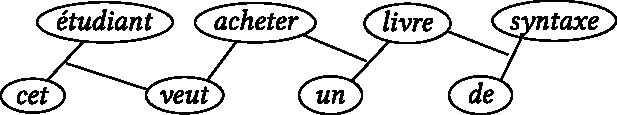
\includegraphics[scale=.75]{figures/ceetudiantveutacheterunlivredesyntaxe.pdf}
% % % \begin{tikzpicture}
% % %   \matrix [matrix of nodes,
% % %            nodes={ConcSet,font=\footnotesize},
% % %            row sep=1em,
% % %            column sep=.333em,
% % %            ampersand replacement=\&] (matrix)
% % %     {
% % %       \& étudiant \& \& acheter \& \& livre \& \& syntaxe\\
% % %       cet \& \& veut \& \& un \& \& de \& \\
% % %     };
% % %     \coordinate (intersection1) at ($ (matrix-1-2) !.5! (matrix-2-1) $);
% % %     \coordinate (intersection2) at ($ (matrix-1-6) !.5! (matrix-2-5) $);
% % %     \coordinate (intersection3) at ($ (matrix-1-8) !.5! (matrix-2-7) $);
% % %     \draw (intersection1) -- (matrix-2-1);
% % %     \draw (intersection1) -- (matrix-1-2);
% % %     \draw (intersection1) -- (matrix-2-3);
% % %     \draw (matrix-2-3)    -- (matrix-1-4);
% % %     \draw (intersection2) -- (matrix-1-4);
% % %     \draw (intersection2) -- (matrix-2-5);
% % %     \draw (intersection2) -- (matrix-1-6);
% % %     \draw (intersection3) -- (matrix-1-6);
% % %     \draw (intersection3) -- (matrix-2-7);
% % %     \draw (intersection3) -- (matrix-1-8);
% % % \end{tikzpicture}         
\caption{\label{fig:}Polygraphe représentant une structure de connexion}
\end{figure}
}


\loupe{Cycle de connexions}{%\label{sec:3.2.24}
    Il peut arriver qu’une unité ABC possède comme sous-unités à la fois AB, BC et AC et que les trois combinaisons A \textrm{${\oplus}$} B, B \textrm{${\oplus}$} C et A \textrm{${\oplus}$} C soient possibles, ce qui donne un \textbf{cycle} (non orienté) de connexions. (On verra, lorsqu’on considérera la dépendance et que les connexions sont orientées, qu’il ne peut pas s’agir d’un cycle orienté ; voir la \sectref{sec:3.3.4} \textit{Structure de dépendance et arbre de dépendance}.) Cette situation se rencontre avec les exemples suivants.

\begin{figure}[H]
\caption{\label{fig:}Structures de connexion avec cycle}
\begin{subfigure}[c]{.5\linewidth}
\centering
\caption{\textit{Marie commet une faute envers Pierre.}}
\begin{tikzpicture}
  \graph [clockwise=3,radius=3em, phase=180, nodes={draw,ellipse,inner sep=1pt,font=\footnotesize\itshape\strut}] {
     {[cycle] {Marie commet}, {une faute}, {envers Pierre}  }
  };
\end{tikzpicture}
\end{subfigure}%
\begin{subfigure}[c]{.5\linewidth}
\centering
\caption{\textit{Je l’ai vu hier à l’école.}}
\begin{tikzpicture}
  \graph [clockwise=3,radius=3em, phase=180, clockwise=3,nodes={draw,ellipse,inner sep=1pt,font=\footnotesize\itshape\strut}] {
     {[cycle] {je l’ai vu}, {hier}, {à l’école} }
  };
\end{tikzpicture}
\end{subfigure}\medskip\\
\begin{subfigure}[c]{.5\linewidth}
\centering
\caption{\textit{la montée du nationalisme en Catalogne}}
\begin{tikzpicture}
  \graph [clockwise=3,radius=3em, phase=180, clockwise=3,nodes={draw,ellipse,inner sep=1pt,font=\footnotesize\itshape\strut}] {
     {[cycle] {la montée}, {du nationalisme}, {en Catalogne} }
  };
\end{tikzpicture}
\end{subfigure}%
\end{figure}


Dans la première phrase, on peut à la fois considérer comme acceptables les unités syntaxiques \textit{commet une faute, commet envers Pierre} et \textit{une faute envers Pierre}. Il s’ensuit que le rattachement du complément \textit{envers Pierre} à \textit{une faute} plutôt qu’à \textit{commet} est incertain, que l’un ou l’autre ne change pas le sens.

La deuxième phrase pose les mêmes problèmes. Il est assez clair que \textit{hier} et \textit{à l’école} sont tous deux des compléments connectés à la construction verbale (\textit{je l’ai vu hier, je l’ai vu à l’école}), mais par ailleurs \textit{hier à l’école} semble aussi fonctionner aussi comme unité syntaxique (\textit{C’est hier à l’école que je l’ai vu} ; \textit{Tu l’as vu} ? \textit{Oui, hier à l’école}.)

Le dernier exemple est du même type encore. S’agit-il du \textit{nationalisme en Catalogne} dont on évoque la montée ou bien du nationalisme dont on considère \textit{la montée en Catalogne}. Peu importe, le sens est à peu près le même et le locuteur n’a pas vraiment les moyens de choisir une connexion plutôt que l’autre. Comme bien sûr \textit{la montée} et \textit{du nationalisme} sont connectés, on a, à nouveau, un cycle potentiel.

Le fait que les trois connexions sont possibles ne signifie pas que les trois connexions coexistent dans la production ou l’analyse de ces exemples. Il est probable que la prosodie produite par le locuteur privilégie une décomposition plutôt qu’une autre et donc une connexion plutôt qu’une autre. On peut penser que, une fois que le destinataire d’un tel énoncé a récupéré une structure connexe satisfaisante, il ne cherche pas à voir s’il pourrait encore la compléter pour obtenir des cycles. En conclusion, nous pensons que la structure syntaxique d’un énoncé peut être potentiellement cyclique, que la manipulation de structures cycliques ne pose pas de problèmes théoriques ou pratiques particuliers, mais nous ne pouvons pas savoir si les locuteurs manipulent ou non des structures syntaxiques cycliques lorsqu’ils produisent ou analysent un énoncé.
}
\section{Analyse en constituants immédiats}\label{sec:3.2.25}

La fragmentation d’un énoncé est à la base de l’\textstyleTermes{analyse en constituants immédiats} (\textstyleTermes{ACI}) initiée par Leonard \citet{bloomfield1933language} et popularisée à la fin des années 1950 par la formalisation qu’en a donnée Noam \citet{chomsky1957syntactic} (voir l’\encadref{fig:3.5.29} sur les \textit{Grammaires de réécriture}). L’ACI fait une hypothèse supplémentaire par rapport à l’approche que nous développons : elle suppose qu’\textbf{une seule fragmentation} d’un énoncé est \textbf{légitime} et que cette unique fragmentation définit les constituants de l’énoncé. L’arbre de fragmentation correspondant est appelé un \textstyleTermes{arbre de constituants}. (Cet arbre est aussi souvent appelé \textit{arbre syntagmatique}, mais nous ne retiendrons pas ce terme qui ne correspond pas à l’usage que nous faisons, à la suite de Saussure, du terme \textit{syntagme}. Voir l’\encadref{fig:3.1.5} \textit{À chacun son syntagme}.)

Henry \citet{gleason1955introduction}, qui est l’un des auteurs qui a défini l’arbre de constituant avec le maximum de rigueur, est explicite sur la nécessité de choisir une fragmentation parmi toutes celles possibles. Le début de sa définition est tout à fait compatible avec la notre : «~Nous pouvons, comme première hypothèse, considérer que chacun des [mots de l’énoncé considéré] a une relation énonçable avec chaque autre mot. Si l’on peut décrire ces interrelations complètement, on aura décrit la syntaxe de l’énoncé dans son entièreté. […] On pourrait commencer par marquer ces paires de mots qui sont ressenties comme ayant les relations les plus étroites.~» Puis sans justification aucune, il ajoute : «~Nous allons aussi imposer la règle que chaque mot peut être marqué comme appartenant à seulement une telle paire.~» Il poursuit en déclarant que la méthode pour trouver la meilleure paire parmi toutes celles possibles est «~le problème de base de la syntaxe~» («~the basic problem of syntax~»), tout en admettant que sa méthode est un peu désordonnée et ne fonctionne pas complètement.

Nous ne partageons pas le point de vue de Gleason et ses contemporains. Nous avons sciemment donné une définition peu restrictive de la notion d’\textit{unité syntaxique}. La plupart des linguistes de la seconde moitié du 20\textsuperscript{e} siècle, et notamment les courants théoriques dit générativistes, issus de l’école chomskyenne, ont défendu que seules les unités qu’ils appellent les \textstyleTermes{constituants syntaxiques} sont des unités syntaxiques légitimes. Nous pensons pour notre part que les constituants syntaxiques sont des unités syntaxiques particulières, certes remarquables, mais qu’il n’y a pas lieu de ne pas considérer les autres unités syntaxiques.

Obtenir une seule décomposition suppose d’avoir des critères beaucoup plus restrictifs que les nôtres pour la définition des unités syntaxiques. Si l’on se place dans ce cadre, on ne peut plus proposer de décomposer \textit{un livre de syntaxe}~à la fois en \textit{un} ${\oplus}$ \textit{livre de syntaxe} et en \textit{un livre} ${\oplus}$ \textit{de syntaxe}. \textbf{Il faut choisir entre les deux décompositions.} Une telle approche suppose par exemple que l’énoncé \textit{Cet étudiant veut acheter un livre de syntaxe} peut être décomposé en \textit{cet étudiant} ${\oplus}$ \textit{veut acheter un livre de syntaxe} à l’exclusion de toute autre décomposition. Il faut donc proposer des critères qui fassent de ces deux fragments les deux seuls fragments acceptables (du point de vue de ces critères). Nous pensons que c’est difficile et, qui plus est, inutile. (Nous discuterons cette question en long et en large au \chapref{sec:3.4}.) Au contraire, en considérant toutes les fragmentations possibles d’un énoncé, on obtient une structure plus riche et finalement plus simple.

Les constituants sont des unités syntaxiques particulières, plus difficiles à caractériser que les unités syntaxiques en général. Il faut pour caractériser les constituants des critères additionnels et notamment faire intervenir la notion de tête dont il sera question au \chapref{sec:3.3}. Dans le \chapref{sec:3.4}, nous verrons qu’il est possible de caractériser, parmi toutes les fragmentations possibles, différentes fragmentations correspondant à un arbre de constituants et que ces fragmentations, accompagnée de l’indication des têtes, permettent de récupérer directement la structure de connexion et donc les autres fragmentations. Nous présenterons en particulier dans l’\encadref{fig:3.4.18} la \textit{Syntaxe X-barre} qui est la version la plus aboutie de l’ACI.

\loupe{Traitement cognitif des connexions}{%\label{sec:3.2.26}
    Bien que cela soit en dehors de notre champ de compétence, nous nous risquons à faire des hypothèses sur le traitement cognitif des connexions. Nous venons de dire que nous pensions que les locuteurs construisent des connexions. La question qui se pose est entre quoi les locuteurs créent-ils des connexions ? Ou dit autrement : quelle instance des connexions les locuteurs construisent-ils ?

    La syntaxe de dépendance traditionnelle répond, à la suite de Tesnière, que les connexions se font entre mots (voir la citation de Tesnière à la \sectref{sec:3.2.8}). La syntaxe générative, si on suit l’analyse en constituants immédiats, répond que les locuteurs connectent les syntaxèmes pour former des constituants de plus en plus gros et que la phrase entière est obtenue par la combinaison de deux constituants que sont le sujet et le groupe verbal. Il est clair pour nous que la syntaxe de dépendance est beaucoup plus proche de la réalité cognitive. On peut néanmoins raisonnablement se demander si toutes les connexions se font entre mots. Existe-t-il des connexions qui s’instancient entre syntaxèmes de mots différents ? Existe-t-il des connexions qui s’instancient entre unités plus larges que le mot ?

    Il est généralement admis que les locuteurs traitent les énoncés de manière \textstyleTermesapprof{incrémentale}, c’est-à-dire au fur et à mesure qu’ils les perçoivent. Une expérience classique est celle des \textstyleTermesapprof{garden paths} (en anglais \textit{to lead somebody up the garden path} signifie ‘mener quelqu’un en bateau’). Lisez les deux phrases suivantes :

    \ea
      \ea \itshape L’espion reconduit à la frontière un diplomate américain.
      \ex \itshape L’espion reconduit à la frontière est un diplomate russe.
      \z
    \z

    Lorsqu’on suit le mouvement des yeux d’un lecteur (on appelle cette méthode l’\textit{eye-tracking}), on observe une saccade régressive sur la deuxième phrase, c’est-à-dire que lorsque le lecteur tombe sur la deuxième forme verbale, \textit{est}, il revient sur la première, \textit{reconduit}, puis revient sur \textit{est}. Ceci tend à prouver que l’analyse est globalement incrémentale, que les mots sont analysés et connectés au fur et à mesure de la lecture, mais que toute analyse qui est infirmée par la suite nécessite un \textstyleTermesapprof{retour en arrière} (angl. \textit{backtracking}) pour détricoter l’analyse en cours.

    Le fait que l’analyse soit globalement incrémentale n’induit pas nécessairement que les syntaxèmes sont systématiquement traités les uns après les autres. Il est probable que les locuteurs traitent le texte par \textbf{petits blocs successifs} et que ces blocs contiennent quelques mots. Donc, d’une part, le locuteur va connecter ces blocs entre eux (voir notamment la stratégie d’analyse de la \encadref{fig:3.5.16} sur le \textit{Flux de dépendances}) et d’autre part, il va les décomposer en syntaxèmes et éventuellement raffiner les connexions.

    La \textbf{prosodie} joue certainement un grand rôle : elle permet, nous pensons, de segmenter une production et d’indiquer pour chacun des segments obtenus qu’il peut être traité indépendamment de la suite et recevoir une structure connexe. La prosodie sert donc (en plus de ses autres fonctions liées à l’expressivité ou au marquage de l’illocution) à guider le traitement de la chaîne parlée par l’interlocuteur.

    Prenons un exemple : \textit{L’autre jour, j’ai rencontré quelqu’un que j’avais pas revu depuis l’école primaire}. Même si \textit{l’autre jour} est détaché et que le reste de l’énoncé forme une unité plus cohésive (un noyau, nous verrons), on n’attend pas d’avoir la totalité du noyau pour connecter \textit{l’autre jour} à la construction verbale. Le complément d’objet direct de \textsc{rencontrer} est un groupe substantival assez long : \textit{quelqu’un que j’avais pas revu depuis l’école primaire}. Même s’il faut avoir traité l’ensemble de ce groupe pour savoir ‘ce que j’ai rencontré’, on n’a pas besoin d’attendre d’avoir traité la relative pour connecter \textit{quelqu’un} à \textit{j’ai rencontré}. Il est d’ailleurs assez probable que l’énoncé soit segmenté prosodiquement de la façon suivante : \textit{l’autre jour {\textbar} j’ai rencontré quelqu’un {\textbar} que j’avais pas revu {\textbar} depuis l’école primaire}, puisque les groupes accentuels tendent à faire autour de 6 syllabes, et qu’il faut que, à chaque frontière de groupe accentuel (marquées ici par {\textbar} ), l’ensemble de ce qui précède reçoive une analyse syntaxique complète. Chacun des quatre groupes prosodiques peut recevoir une analyse complète indépendamment des autres groupes, puis être connecté aux autres, ce qui donne quelque chose comme ça :

    \begin{figure}[H]
    \begin{tikzpicture}
    \node at (0,0)  [ConcSet,font=\small] (A) {\textit{l’autre jour}};
    \node at (3,-1) [ConcSet,font=\small] (B) {\textit{j’ai rencontré quelqu’un}};
    \node at (6,-2) [ConcSet,font=\small] (C) {\textit{que j’avais pas revu}};
    \node at (9,-3) [ConcSet,font=\small] (D) {\textit{depuis l’école primaire}};
    \path [draw] (A.north east) edge [out=45, in=80] (B)
                 (B.north east) edge [out=45, in=80] (C)
                 (C.north east) edge [out=45, in=80] (D);
    \end{tikzpicture}
    \caption{Structure de connexion induite par la prosodie}
    \end{figure}

    Nous pouvons dire pour conclure que la représentation de l’organisation syntaxique d’un énoncé par une structure de connexions présente des avantages pour qui voudrait étudier plus avant le traitement cognitif de la parole et de la lecture, permettant de rendre compte d’une connexion à différents niveaux de granularité, d’attribuer des analyses à n’importe quelle portion d’un énoncé et de construire la structure d’un énoncé de manière incrémentale.
}
\exercices{%\label{sec:3.2.27}
    \exercice{1} 
    \begin{enumerate}[label=\alph*.]
    \item Expliquez quelles contraintes agissent sur la réalisation du sens ‘rapide’ dans les deux phrases suivantes :
      \begin{enumerate}[label=(\arabic*)]
      \item   \textit{{Zoé a jeté un coup d’œil} \textbf{{rapide}}  {dans la pièce.}}
      \item   \textit{{Zoé a regardé} \textbf{{rapidement}}  {dans la pièce}.}
      \end{enumerate}
    \item Quelles contraintes agissent sur la réalisation de ‘épée’ dans les deux phrases suivantes ?
     \todo[inline]{Continue the numbering: (3) and (4)}
     \begin{enumerate}[label=(\arabic*)]
      \item \textit{{Manier une} \textbf{{épée}}  {peut être dangereux.}}
      \item \textit{{Le maniement d’une} \textbf{{épée}}  {peut être dangereux}.}
      \end{enumerate}
    \end{enumerate}
    \exercice{2} Comparer les paradigmes de commutation de la position sujet du verbe \textsc{plaire} et de la position objet du verbe \textsc{aimer}. Quelles sont les (petites) différences ?
    \begin{enumerate}[label=(\arabic*)]
       \item \textit{\textbf{{Le chocolat}}  {plaît à Jean.}}
       \item \textit{{Jean aime} \textbf{{le chocolat}}.}
    \end{enumerate}
    \exercice{3} Donner la liste des unités syntaxiques autonomisables (c’est-à-dire plus grandes ou égales à un mot) de l’énoncé :
    \begin{enumerate}[label=(\arabic*)]
        \item {Cet étudiant veut acheter un livre de syntaxe}
    \end{enumerate}
    \exercice{4} En utilisant le test d’autonomisabilité illocutoire, déterminer les unités syntaxiques autonomisables des énoncés suivants et en déduire la structure de connexion correspondante.
    
    \begin{enumerate}[label=(\arabic*)]
    \item \textit{Ça a commencé bien des années plus tard}.
    \item \textit{le plus haut mur du monde}.
    \end{enumerate}
    \exercice{5} On propose la structure de connexion suivante pour \textit{Le chat dort sur le lit}.

    \begin{center}
    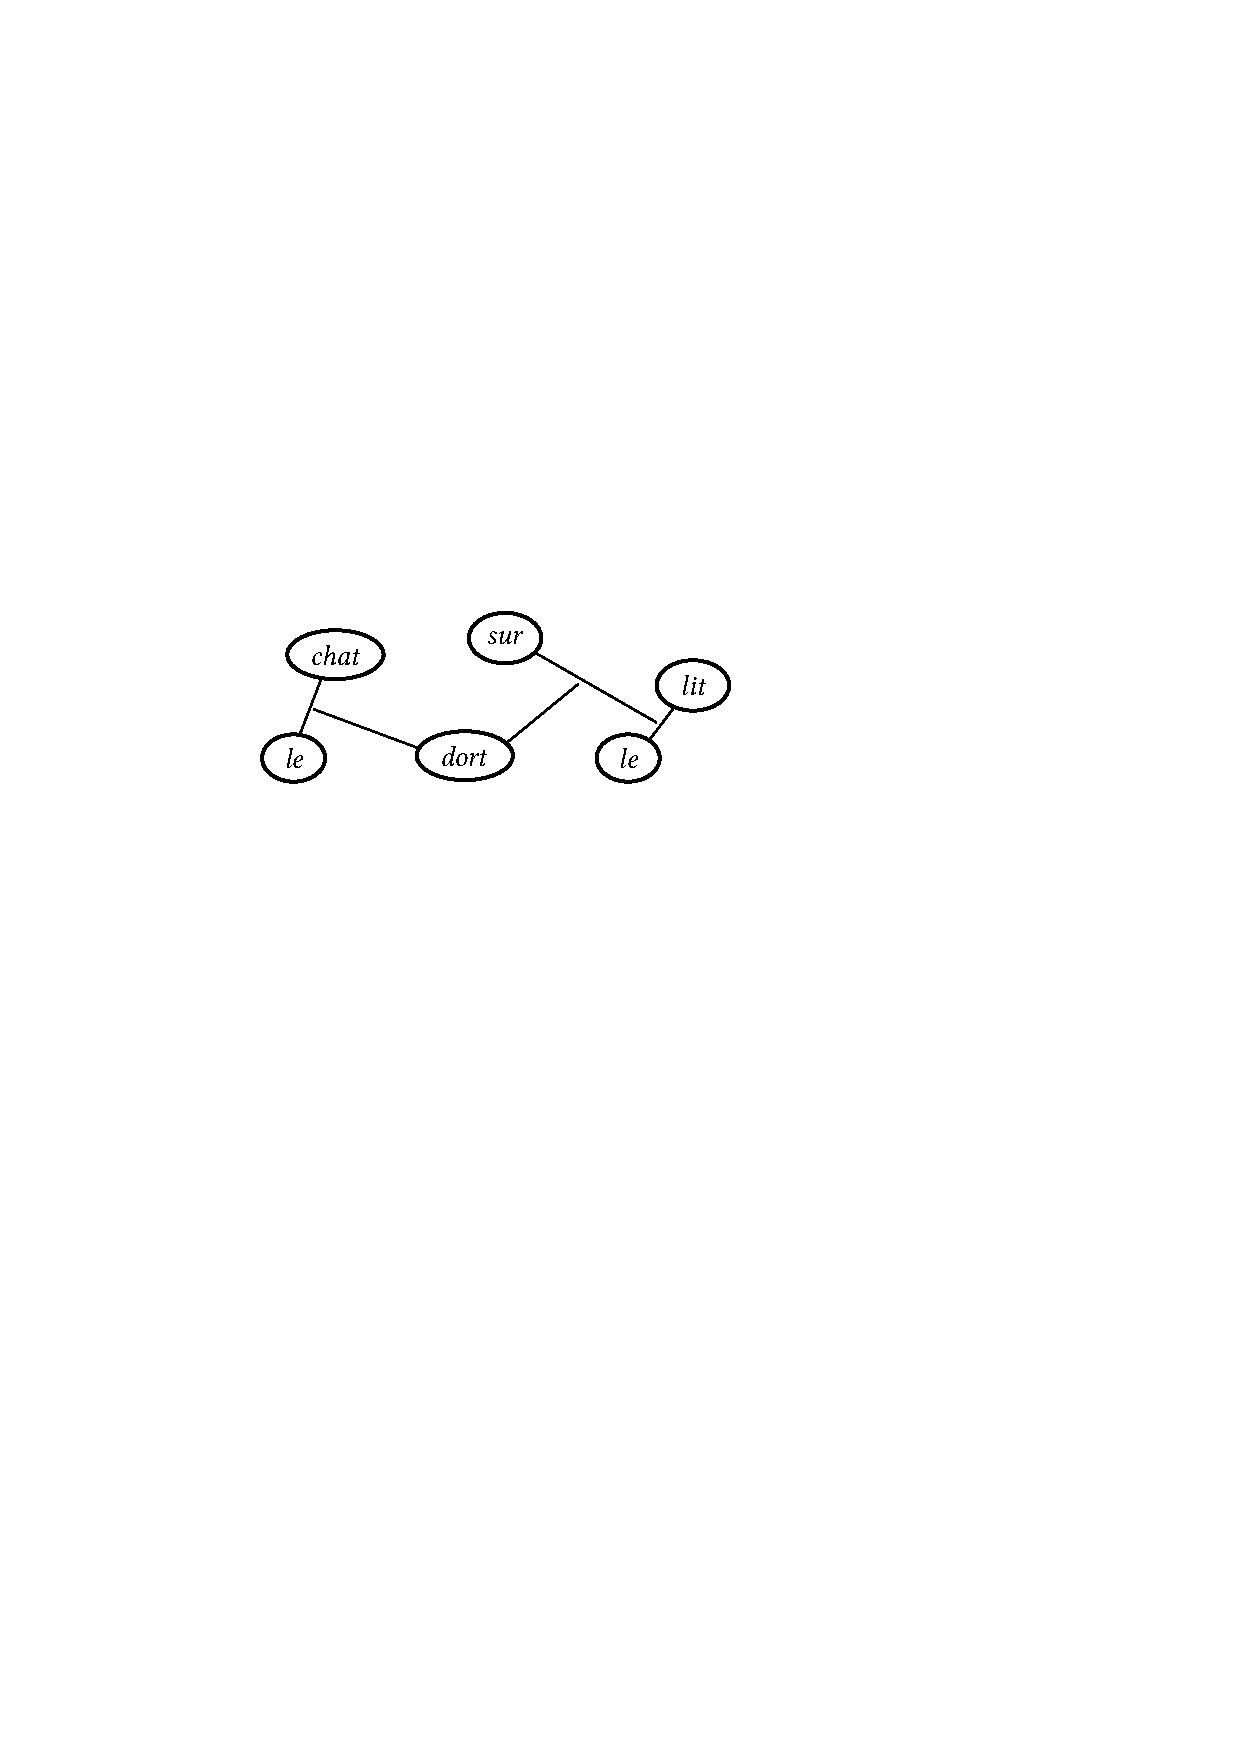
\includegraphics[scale=.75]{lechatdortsurlelit.pdf}
% %     \begin{tikzpicture}
% %       \matrix (matrix) [matrix of nodes,
% %                         nodes={ConcSet},
% %                         row sep=1em, 
% %                         column sep=1em,
% %                         ampersand replacement=\&]
% %         {
% %           \& chat \& \& sur \& \& lit\\
% %           le \& \& dort \& \& le \& \\
% %         };
% %       \coordinate (intersection1) at ( $ (matrix-2-1) !.5! (matrix-1-2) $ );
% %       \coordinate (intersection2) at ( $ (matrix-2-5) !.5! (matrix-1-6) $ );
% %       \coordinate (intersection3) at ( $ (matrix-1-4) !.5! (intersection2) $ );
% %       \draw (matrix-2-1)    -- (matrix-1-2);
% %       \draw (intersection1) -- (matrix-2-3)
% %                             -- (intersection3);
% %       \draw (matrix-1-4)    -- (intersection2);
% %       \draw (matrix-1-6)    -- (matrix-2-5);
% %     \end{tikzpicture}
    \end{center}

    Cette structure est donnée sous forme de polygraphe (voir \encadref{fig:3.2.23}).
    
    \begin{enumerate}[label=\alph*.]
    \item Quelles sont les unités qu’on peut déduire de cette structure ?
    \item À quels critères répond cette structure de connexion ?
    \item Peut-on raffiner les connexions de cette structure ? En utilisant quels critères ?
    \end{enumerate} 
}
\lecturesadditionnelles{%\label{sec:3.2.28}
    L’organisation de nos chapitres doit beaucoup aux travaux d’Igor Mel’čuk. Celui-ci considère 3 types de critères pour définir la structure syntaxique : les critères A décident si deux mots se combinent entre eux, les critères B lequel des deux mots est la tête du syntagme qu’ils forment, les critères C quelle est la relation qui les unit. Le présent chapitre est ainsi consacré aux combinaisons et donc aux critères A. Nous avons étendu l’analyse de Mel’čuk en ne limitant pas la connexion aux combinaisons de mots. Les critères B seront étudiés au \chapref{sec:3.3} sur \textit{Tête et dépendance}. Les critères C seront abordés plus tard, dans le \chapfuturef{18} sur \textit{Les relations syntaxiques.}

    L’autonomisabilité prosodique~et plus généralement la relation entre une structure de dépendances syntaxique et la structure prosodique a été étudiée par Piet Mertens dans sa thèse en 1987. Pour un travail plus récent, on pourra consulter son article de 2008. Pour un travail précurseur sur les liens entre prosodie et syntaxe de dépendance, citons le travail d’Henri Weil (1844) sur lequel nous reviendrons.

    Lucien Tesnière utilise des bulles dans ses représentations syntaxiques. Une formalisation des arbres à bulles est proposée par Kahane (1997). La définition de la structure de connexion par raffinement d’une fragmentation est proposée par Gerdes \& Kahane (2011). La définition de la connexion comme une classe d’équivalence de combinaisons est développée dans Kahane (2018). Le lien historique entre connexion et analyse en constituants immédiats, chez Henry A. Gleason comme chez ses prédécesseurs, est étudié par Mazziotta \& Kahane (2017). Timothy Osborne et ses collègues ont consacré un article aux catenae en 2012.

    Sur le traitement cognitif de la syntaxe, on consultera les travaux précurseurs de Janet D. Fodor et de son étudiante Lyn Frazier. Dans leur article de 1978, elles défendent l’idée que les énoncés sont traités par petits paquets d’environ six mots qui sont ensuite connectés entre eux. Cette étude est suivie en 1982 et 1994 d’une analyse du traitement des phrases avec garden-path par l’analyse des mouvements oculaires, où il est défendu que l’énoncé n’est pas réanalysé, mais que le destinataire répare sa première analyse après avoir identifié la source de l’erreur.
    
    \FurtherReading{3-2}
    \todo[inline]{citation of PhD theses is strange}\noindent
}
\citations{%\label{sec:3.2.29}
    {\bfseries Citations de la \sectref{sec:3.2.25}.}

    \citet[129--130]{gleason1955introduction} :

    \begin{quote}
    We may, as a first hypothesis, consider that each of [the words of the considered utterance] has some statable relationships to each other word. If we can describe these interrelationships completely, we will have described the syntax of the utterance in its entirety. […] We might start by marking those pairs of words which are felt to have the closest relationship.~[…]~We will also lay down the rule that each word can be marked as a member of only one such pair.~
    \end{quote}
}
\corrections{%\label{sec:3.2.30}
\corrigé{1} 
\begin{enumerate}[label=\alph*.]
\item Dans le premier cas, \textit{rapide} se combine avec la locution nominale \textit{coup d’œil}, ce qui explique la réalisation comme adjectif. Dans le deuxième cas, la combinaison a lieu avec le verbe \textsc{regarder}, ce qui entraine la réalisation par l’adverbe \textit{rapidement}.

\item Dans le premier cas, \textit{une épée} est le complément d’objet direct de la forme infinitive du verbe \textsc{manier}. Dans le deuxième cas, \textit{une épée} est le complément du nom \textit{maniement~}; dans ce cas, \textit{une épée} doit d’abord se combiner avec la préposition \textsc{de} avant de se combiner avec \textit{maniement}.
\end{enumerate}

\corrigé{2} Les deux positions acceptent des groupes substantivaux, des infinitives (\textit{lire le soir}) et des propositions complétive (\textit{qu’il pleuve le matin}). On observe deux différences dans les paradigmes. D’une part, les pronoms sujets et objets sont différents : \textit{\textbf{il} plaît à Marie} vs \textit{Marie} \textbf{\textit{l’}}\textit{aime}. D’autre part, la position sujet accepte des infinitives en \textit{de~}: \textit{\textbf{De lire le soir} plaît à Marie} vs *\textit{Marie aime de lire le soir}.

\corrigé{3} Les unités syntaxiques autonomisables de cet énoncé sont :

\begin{itemize}
\item les 8 mots : \textit{cet, étudiant, veut, acheter, un, livre, de, syntaxe~};
\item 4 segments de deux mots : \textit{cet étudiant, veut acheter, un livre, de syntaxe~};
\item 3 segments de trois mots : \textit{cet étudiant veut, acheter un livre, livre de syntaxe~};
\item 3 segments de quatre mots : \textit{cet étudiant veut acheter, veut acheter un livre, un livre de syntaxe~};
\item 1 segment de cinq mots : \textit{acheter un livre de syntaxe~};
\item 2 segments de six mots : \textit{cet étudiant veut acheter un livre, veut acheter un livre de syntaxe~};
\item l’énoncé complet : \textit{cet étudiant veut acheter un livre de syntaxe}.
\end{itemize}

\corrigé{4} 
\begin{enumerate}[label=\alph*.]
\item \textit{bien des années plus tard} forme un syntagme, puisqu’il peut être la réponse à la question «~\textit{Ca a commencé quand} ?~». À la même question, on peut répondre \textit{des années plus tard}, \textit{bien plus tard} ou \textit{plus tard}, voire juste \textit{tard}, mais pas \textit{bien des années}, \textit{bien}, \textit{des années} ou \textit{plus}. On en déduit que \textit{bien} et \textit{des années} se combinent avec \textit{plus tard}. Il est plus difficile de déterminer si \textit{bien} et \textit{des années} se combinent avec \textit{plus} ou \textit{tard}, puisque ni \textit{des années plus}, ni \textit{des années tard} n’est acceptable. On peut néanmoins remarquer qu’on trouve un groupe substantival avec \textit{plus} dans d’autres contextes : \textit{Il habite un étage plus haut~}; \textit{Fais-le deux centimètres plus large}. Par contre, on ne peut jamais combiner un groupe substantival avec \textit{tard} sans la présence de \textit{plus}, ce qui nous permet de conclure que \textit{des années} se combine avec \textit{plus}. Si \textit{bien} peut se combiner aussi bien avec \textit{plus} que \textit{tard}, il semble, au vu du sens, que c’est avec \textit{plus} qu’il se combine ici.
   

\begin{center}
\begin{tikzpicture}[every node/.style={font=\footnotesize,inner sep=1pt}]
 \node at (0,0) (A) [draw,circle,font=\itshape\strut] {ça};
 \node [right=1em of A] (B) [draw,circle,font=\itshape\strut] {a};
 \node [right=1em of B] (C) [ConcSet] {commencé};
 \node [right=1em of C] (D) [ConcSet] {tard};
 \node [right=1em of D] (E) [ConcSet] {plus};
 \node [above right=\baselineskip and 1em of E] (F) [ConcSet] {des};
 \node [right=1em of F] (G) [ConcSet] {années};
 \node [below right=\baselineskip and 1em of E] (H) [ConcSet] {bien};
 
 \node [fit = (F) (G),draw,ellipse,inner sep=0pt] (FG) {};
 \draw (A) -- (B) -- (C) -- (D) -- (E) -- (FG);
 \draw (F) -- (G);
 \draw (E) -- (H);
\end{tikzpicture}
\end{center}


\item La fragmentation du syntagme \textit{le plus haut mur du monde} pose plusieurs problèmes. Nous avons déjà traité le cas des adjectifs épithètes et expliqué pourquoi \textit{le haut} n’est pas un fragment acceptable. Mais c’est plus compliqué avec \textit{le plus haut}, puisqu’on a \textit{le mur le plus haut}. On peut argumenter que \textit{le} dans \textit{le plus haut mur} est bien l’article, car il commute avec un possessif : \textit{son plus haut mur}, \textit{mon plus vieil ami}. Ce qui n’est pas le cas qu’en \textit{le plus haut} forme une unité syntaxique et un groupe adjectival postposé au nom : *\textit{le mur notre plus haut}. On aurait donc la structure de connexion suivante pour \textit{le plus haut mur} :

\begin{center}
\begin{tikzpicture}
\matrix (matrix) [matrix of nodes, 
                  nodes = {ConcSet, minimum width=3em},
                  ampersand replacement=\&,
                  row sep=1em,
                  column sep=.33em,
                  inner sep = 0pt,
                  font=\small]
  { \& haut \& \& mur\\
      plus \& \& le\\  
  };
\draw (matrix-2-1) -- (matrix-1-2) -- (matrix-1-4) -- (matrix-2-3);
\end{tikzpicture}
\end{center}

Mais on peut aussi accepter que dans cette construction \textit{le} joue un double rôle : à la fois article défini (\textit{le mur}) et marqueur du superlatif (le plus), ce qui donne une structure cyclique.

\begin{center}
\begin{tikzpicture}
\matrix (matrix) [matrix of nodes, 
                  nodes = {ConcSet, minimum width=3em},
                  ampersand replacement=\&,
                  row sep=1em,
                  column sep=.33em,
                  inner sep = 0pt,
                  font=\small] 
  {
    \& haut \& \& mur\\
    plus \& \& le\\
  };
\draw (matrix-2-1) -- (matrix-1-2) -- (matrix-1-4) -- (matrix-2-3) -- (matrix-2-1);
\end{tikzpicture}
\end{center}

%%[Warning: Draw object ignored]
%%[Warning: Draw object ignored]


Un autre problème d’analyse vient du modifieur \textit{du monde}. Il ne s’agit pas d’un complément du nom \textit{mur}, puisque \#\textit{mur du monde}, s’il est acceptable, n’a pas le sens requis et surtout on a \textit{le mur le plus haut du monde}. De même, \textit{du monde} n’est pas un modifieur de l’adjectif, car l’absence du superlatif donne un sens inapproprié : \#\textit{le haut mur du monde}. Donc, bien que le fragment \textit{le plus du monde} soit inacceptable, nous pouvons considérer que la présence du modifieur du monde est validé par la présence du superlatif et que les deux sont donc connectés.
\end{enumerate}

\todo[inline]{No break after title}
\corrigé{5} 
\begin{enumerate}[label=\alph*.]
\item Les unités induites sont les mots, ainsi que \textit{le lit, sur le lit, le chat, le chat dort, dort sur le lit} et la phrase entière.
\item Ces unités obéissent aux critères d’autonomisabilité. En particulier, \textit{sur} ne peut apparaître sans son complément \textit{le lit}.
\item On peut raffiner la structure en utilisant le critère distributionnel. Nous verrons au chapitre suivant qu’il y a de bonnes raisons de considérer la combinaison \textit{dort} \textrm{${\oplus}$} \textit{sur}. Il est moins facile de raffiner les connexions mettant en jeu une unité déterminant-nom comme \textit{le chat} ou \textit{le lit}.
\end{enumerate}}
